\documentclass[a4paper]{report}
\usepackage[french]{babel}
\usepackage[utf8]{inputenc}
\usepackage{graphicx}
\usepackage[colorinlistoftodos]{todonotes}
\usepackage{amsthm}
\usepackage{amsmath}
\usepackage{amsfonts}
\usepackage{tabularx}
%\usepackage[nottoc, notlof, notlot]{tocbibind}
\usepackage{charter}
\usepackage[T1]{fontenc}
\usepackage{url}
%\usepackage{geometry}
\usepackage{enumitem}
\usepackage{hyperref}






\newtheoremstyle{break}  % follow `plain` defaults but change HEADSPACE.
  {\topsep}   % ABOVESPACE
  {\topsep}   % BELOWSPACE
  {}  % BODYFONT
  {0pt}       % INDENT (empty value is the same as 0pt)
  {\bfseries} % HEADFONT
  {.}         % HEADPUNCT
  {\newline}  % HEADSPACE. `plain` default: {5pt plus 1pt minus 1pt}
  {}          % CUSTOM-HEAD-SPEC
\theoremstyle{break}

\newtheorem{defin}{Définition}
\def\definautorefname{Définition}
\newtheorem{exem}{Exemple}
\def\exemautorefname{Exemple}




\newtheoremstyle{breakplain}  % follow `plain` defaults but change HEADSPACE.
  {\topsep}   % ABOVESPACE
  {\topsep}   % BELOWSPACE
  {\itshape}  % BODYFONT
  {0pt}       % INDENT (empty value is the same as 0pt)
  {\bfseries} % HEADFONT
  {.}         % HEADPUNCT
  {\newline}  % HEADSPACE. `plain` default: {5pt plus 1pt minus 1pt}
  {}          % CUSTOM-HEAD-SPEC
\theoremstyle{breakplain}
\newtheorem{theo}{Théorème}
\def\theoautorefname{Théorème}
\def\lemautorefname{Lemme}
\newtheorem{lem}{Lemme}

\title{Préparation au mémoire --- MEMO-F-403\\Ordonnancement de systèmes à criticité mixte et méthodes formelles}
\author{Simon \textsc{Picard}}
\date{22 mai 2015}

\begin{document}
%\maketitle
\begin{titlepage}
\begin{center}
\textbf{UNIVERSIT\'E LIBRE DE BRUXELLES}\\
\textbf{Faculté des Sciences}\\
\textbf{Département d'Informatique}
\vfill{}\vfill{}
%\begin{center}
{\Huge  Ordonnancement de systèmes à criticité mixte et méthodes formelles}
%\end{center}
{\Huge \par}
\begin{center}{\LARGE Simon \textsc{Picard}}\end{center}{\Huge \par}
%\vfill{}\vfill{}\vfill{}\vfill{}\vfill{}
\vfill{}

\includegraphics[width=\textwidth-2cm]{images/sceau-b-quadri.jpg}
\vfill{}
\begin{flushright}{\large \textbf{Promoteurs :}}\hfill{}{\large Mémoire présenté en vue de}\\
{\large Prof. Gilles Geeraerts}\hfill{}{\large l'obtention du grade de}\\{\large Prof. Joël Goossens}
\hfill{}{\large Master en Sciences Informatiques}\end{flushright}{\large\par}
\vfill{}\vfill{}\enlargethispage{2cm}
\textbf{Année académique 2015~-~2016}
\end{center}
\end{titlepage}

\tableofcontents
\chapter{État de l'art}
Ce document a été réalisé dans le cadre du second cycle d'études à l'ULB en science informatique. C'est la première partie du travail total que représente le mémoire. Le but est de se lancer dans la rédaction d'un travail de fin d'études porté sur un sujet choisi par l'étudiant, qui comprend en premier lieu un état de l'art et ensuite un travail personnel sur le sujet défini à la fin de ce papier. En l'état, ce document contient la partie état de l'art. Cette dernière est donc portée essentiellement sur la recherche bibliographique, la lecture et la compréhension. Ce travail est réalisé sous la direction des professeurs Gilles Geeraerts et Joël Goossens.\\

Ce chapitre présente l'état de l'art ayant pour sujet deux problèmes différents de deux domaines différents de l'informatique. Premièrement, le chapitre se concentre sur l'ordonnancement à criticité mixte, pour se faire, il faut commencer par introduire l'ordonnancement classique, puis une explication informelle de ce type d'ordonnancement est donnée pour enfin terminer par le formalisme de celui-ci. Dans un second temps, le problème de l'accessibilité est présenté, en commençant par fournir certaines notions de base, ensuite en exposant un formalisme pour finir par expliquer la notion d'antichaîne. Par la suite, l'interaction entre ces deux problèmes est mise au clair. Et pour finir, les contributions qui seront faites dans ce mémoire sont détaillées.

\section{Ordonnancement de systèmes à criticité mixte}
\subsection{Notions élémentaires}
L'un des domaines majeurs de l'informatique théorique actuelle est celui de l'ordonnancement, il s'agit d'organiser dans le temps la réalisation de différents travaux compte tenu de contraintes temporelles. Pour s'exécuter, ces travaux ont besoin d'avoir accès à une ou plusieurs ressources partagées entre eux. En pratique, une fois qu'un travail est généré, il possède un temps d'exécution et une échéance. Dans la plupart des cas, on parle de système comprenant une série de travaux, le but est alors d'agencer ces différents travaux de sorte qu'ils ne ratent pas leurs échéances, il faut partitionner la ou les ressources partagées entre les travaux. L'objet de cette sous-section est de définir un certain modèle pour ce problème ainsi que d'introduire différentes notions de la théorie de l'ordonnancement.
\subsubsection{Modèle}
Pour permettre l'ordonnancement d'un système, un certain formalisme a été défini, cette partie le présente.\\

Commençons par une notion fondamentale, le travail. Il s'agit d'un ensemble d'opérations à effectuer nécessitant de prendre possession de la ou une des ressources partagées.

\begin{defin}[Travail \cite{goossens2014os}]
Un travail est représenté par un triplet : 
\begin{center}
$J_i = (r_i, d_i, c_i)$
\end{center}
\begin{itemize}
\item $r_i \in \mathbb{N}^{+}$ est l'instant auquel $J_i$ est généré.
\item $d_i \in \mathbb{N}^{+}$ est l'échéance absolue de $J_i$, c'est-à-dire le moment avant lequel le travail doit impérativement avoir été exécuté complètement. On assume que $d_i > r_i$
\item $c_i \in \mathbb{N}^{+}$ définis la durée d'exécution du travail.
\end{itemize}
Le travail $J_i$ doit donc recevoir $c_i$ unités de processeur durant l'intervalle $[r_i, d_i)$. $[a,b)$ est l'intervalle entre $a$ et $b$, $a$ est inclus et $b$ ne l'est pas. \\
En général, on parle d'instance $I$, il s'agit d'un ensemble de travaux : $ I = \{J_1, J_2, ...\} $
\end{defin}

Souvent, le programme à exécuter possède une partie d'opération récurrente, en particulier on considère les tâches périodiques et sporadiques.

\begin{defin}[Tâche périodique \cite{goossens1999scheduling}]
Une tâche périodique génère donc un nombre infini de travaux, elle est représentée par un quadruple :
\begin{center}
$\tau_i = (O_i, T_i, D_i, C_i)$
\end{center}
\begin{itemize}
\item $O_i \in \mathbb{N}^{+}$ est le décalage de la tâche, l'instant auquel le premier travail de la tâche est généré.
\item $C_i \in \mathbb{N}^{+}$ définis la durée d'exécution d'un travail généré par la tâche.
\item $D_i \in \mathbb{N}^{+}$ est l'échéance relative de la tâche, c'est donc le laps de temps entre la génération d'un travail et son échéance absolue.
\item $T_i \in \mathbb{N}^{+}$ est la périodicité de la tâche, c'est-à-dire l'intervalle entre deux générations de travail.
\end{itemize}
Le $k^{e}$ travail $J_{i,k}$ de la tâche $\tau_i$ est donc généré à l'instant $O_i + (k-1)*T_i$ et a pour échéance  $O_i+(k-1)*T_i+D_i$ .
\end{defin}
\begin{defin}[Tâche sporadique \cite{goossens1999scheduling}]
Une tâche sporadique possède le même modèle que la tâche périodique, la différence est que $T_i$ ne représente plus la périodicité, mais le temps minimal entre deux générations de tâche. La tâche sporadique est donc imprévisible.
\end{defin}


On définit ensuite une série caractéristique \cite{goossens1999scheduling} qu'une tâche peut avoir :
\begin{itemize}
\item Une tâche à échéance implicite est une tâche où l'échéance correspond à la période, $D_i = T_i\ \forall i$
\item Une tâche à échéance contrainte est une tâche où l'échéance est inférieure ou égale à la période, $D_i \le T_i\ \forall i$
\item Une tâche à échéance arbitraire est une tâche où il n'y a pas de contraintes en la période et l'échéance de celle-ci.
\end{itemize}
On définit ensuite, sur un système de plusieurs tâches $\tau = \{\tau_1, \tau_2, ...\}$
\begin{itemize}
\item Un système de tâche est synchrone si toutes ses tâches ont un décalage nul, $O_i = 0\ \forall i$
\item Asynchrone sinon.
\end{itemize}

\subsubsection{Ordonnancement}
Une stratégie d'ordonnancement est un algorithme permettant le partage d'une ou plusieurs ressources entre plusieurs parties dont elles font la requête de manière simultanée et asynchrone \cite{goossens2014os}. Les ordonnanceurs sont utilisés par exemple dans un système d'exploitation, dans les disques durs, dans les routeurs internet ... Le but d'un ordonnanceur classique est d'éviter le gaspillage de ressource et de partager cette dernière de manière équitable entre ceux qui le demandent. Dans un ordonnanceur temps réel, une contrainte de temps doit être respectée, il faut que les processus se terminent avant leurs échéances, ce type d'ordonnanceur est largement utilisé dans les systèmes embarqués, par exemple dans un cardiostimulateur.\\

À l'heure actuelle, les constructeurs de système embarqué ont tendance à implémenter plusieurs fonctionnalités sur une même plateforme pour réduire les coûts, la chaleur, l'alimentation... Malheureusement, un tel partage de ressource peut mener à des interférences entre les différents clients, on cherche donc à savoir si oui ou non, un tel ensemble de clients peuvent partager une ressource sans qu'il y ait de moments où un client n'a pas accès à cette ressource alors qu'il en a besoin.\\
Typiquement, on parle d'ordonnancement d'un processeur, on divise donc le temps d'exécution disponible grâce aux coups d'horloge, définissant le temps entre deux coups d'horloge successifs comme une unité de temps. L'ordonnanceur peut être préemptif, c'est-à-dire qu'il peut interrompre un travail pour en ordonnancer un autre, ou non.\\

Dans ce document, nous nous concentrerons sur les algorithmes d'ordonnancement préemptif sur un monoprocesseur à vitesse unitaire.\\

L'algorithme d'ordonnancement devra choisir parmi plusieurs travaux lequel pourra jouir de la puissance du processeur.  Pour ce faire, il utilisera un système de priorité clair et défini, chaque travail possédera une priorité et, en fonction de celle-ci, l'ordonnanceur pourra partager le temps de calcul entre les travaux. Il existe trois classes d'algorithme d'ordonnancement \cite{goossens2014os} :

\begin{itemize}
\item Priorité fixe au niveau des tâches (Fixed Task Priority, FTP) : il s'agit d'un ordonnancement où chaque tâche s'est vue attribuer une priorité avant l'exécution du système. Chaque travail hérite ensuite de la priorité de la tâche qui l'a générée.
\item Priorité fixe au niveau des travaux (Fixed Job Priority, FJP) : chaque travail reçoit un niveau de priorité lorsqu'il est généré, celui-ci restera constant pour toute la vie du travail. Dès lors, différents travaux d'une même tâche peuvent avoir une priorité différente.
\item Priorité dynamique (Unrestructed Dynamic Priority, DP) : il s'agit du cas général où aucune contrainte ne s'applique à l'assignation des priorités aux travaux. En règle générale, cette nouvelle ligne conduite signifie qu'un travail va changer de priorité durant son existence.
\end{itemize}
On remarque que ces différentes classifications s'incluent elles-mêmes, en effet, FTP fait partie de la classe FJP qui est elle-même dans la classe DP.\\

L'ordonnancement est donc avant tout une certaine assignation de priorité, de manière générale on considère que la valeur de la priorité attribuée à un travail est un naturel et est inversement proportionnel à sa priorité. Si deux travaux ont une même priorité, il faudra choisir de manière déterminée lequel sera ordonnancé. On définit donc la relation de priorité par le symbole $\succ$, par exemple : $\tau_i \succ \tau_j$, ici $\tau_i$ a une priorité supérieure à celle de $\tau_j$.\\

\begin{defin}[Fonction de priorité \cite{santy2012ordonnancement}]
Formellement, une fonction de priorité $\pi$ assigne à toute tâche $\tau_i$ d'un système de $n$ tâches $\tau$ (respectivement à tout travail $J_i$ d'une instance de $m$ travaux $I$) un nombre entier $\pi(\tau_i)$ (respectivement $\pi(J_i)$) compris entre $1$ et $n$ (respectivement $m$) qui représente de manière inversement proportionnelle la priorité de la tâche (respectivement du travail).
\begin{center}
$\pi : \tau \rightarrow \{0,...,n \}$\\
(Respectivement $\pi : I \rightarrow \{0,...,m \}$)\\
$\pi(\tau_i) < \pi(\tau_j) \Leftrightarrow \tau_i \succ \tau_j$\\
(Respectivement $\pi(J_i) < \pi(J_j) \Leftrightarrow J_i \succ J_j$)
\end{center}
\end{defin}

En temps réel, l'ordonnancement se porte en général sur un système de tâche, on souhaite prouver si oui ou non un tel ensemble satisfait les conditions introduites par ce mode, deux nouvelles caractéristiques en émergent \cite{goossens2014os} :

\begin{itemize}
\item La faisabilité d'un système de tâche est vérifiée s'il existe un certain partage du temps de calcul entre les différents travaux de sorte que chacun d'entre eux ait pu exécuter toutes leurs actions sans rater leur échéance.
\item Un système de tâche est ordonnançable avec un certain algorithme d'ordonnancement si celui-ci permet d'agencer les travaux de sorte que chacun d'entre eux ait pu exécuter toutes leurs actions sans rater leur échéance.
\end{itemize}

Une définition analogue peut être faite pour une collection de travaux.\\
Il est à noter qu'il est possible qu'un système de tâche soit faisable, mais pas ordonnançable dans certains cas. Ces deux notions sont souvent liées à celle de l'utilisation qui représente la charge de travail du processeur, la quantité de travail effectué par rapport au temps dont il dispose pour le faire.

\begin{defin}[Utilisation \cite{goossens2014os}]
L'utilisation d'une tâche est définie par la fonction $U(\tau_i) = C_i/T_i$.\\
L'utilisation d'un système est la somme des utilisations des tâches le composant : $U(\tau) = \underset{\tau_i \in \tau}{\sum} (\tau_i)$
\end{defin}

Pour clôturer cette sous-section, un algorithme d'ordonnancement monoprocesseur est présenté. Il s'agit d'un algorithme à priorité statique au niveau des travaux (FJP) : EDF (Earliest Deadline First). Celui-ci attribue à chacun des travaux une priorité relative à leurs échéances absolues, au plus elles sont proches, au plus prioritaire est le travail. Formellement, on obtient $d_i < d_j \Leftrightarrow J_i \succ J_j$ et en cas d'égalité, $d_i = d_j \wedge i < j \Leftrightarrow J_i \succ J_j$.

\begin{theo}[\cite{goossens2014os}]
Si une collection de travaux est faisable, alors elle est ordonnançable avec EDF.
\end{theo}

EDF est donc un algorithme optimal pour un système de tâche à échéance implicite, synchrone ou asynchrone. Un algorithme est optimal si l'agencement qu'il génère permet d'ordonnancer tout système de tâche d'un certain type.

\begin{theo}[\cite{liu1973scheduling}]
Pour un système de tâche périodique à échéance implicite $\tau$, celui-ci est faisable si et seulement si $U(\tau) \leq 1$
\end{theo}

\begin{figure}[h]
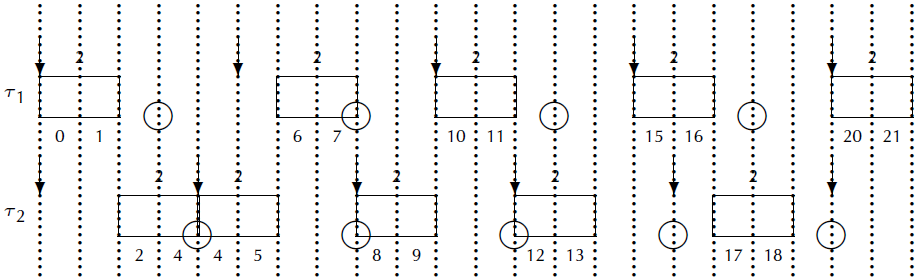
\includegraphics[width = \textwidth]{images/schedexample.png}
\caption{Représentation graphique d'un exemple d'ordonnancement par EDF \cite{goossens2014os}}
\label{edfsched}
\end{figure}

Il sera fréquent de représenter l'ordonnancement de travaux de manière graphique, la figure~\ref{edfsched} en est un exemple, ici il s'agit d'un système de deux tâches.
\begin{center}
$ \tau_1 = (0, 5, 3, 2) $\\
$ \tau_2 = (0, 4, 4, 2) $
\end{center}
Sur l'image :
\begin{itemize}
\item Chaque colonne en pointillé représente une unité de temps.
\item Une tâche est représentée sur une ligne
\item La flèche vers le bas représente la période de la tâche et donc le moment où le travail est généré
\item Un rond représente l'échéance d'un travail
\item Un carré représente l'exécution d'un travail durant une unité de temps
\end{itemize}

\subsection{Criticité mixte}
\subsubsection{Définition informelle}
Le problème de criticité mixte est un problème d'ordonnancement. Pour rappel, il s'agit donc de gérer le partage d'un ensemble de ressources communes entre plusieurs clients.\\

Dans cette sous-section, nous nous penchons sur un problème plus précis : celui de la certification, dont le but est de prouver qu'un système est ordonnançable.\\

Précédemment, il a été présenté l'ordonnancement de travaux classique, ici on en déduit un nouveau problème où les clients pourraient avoir une importance plus ou moins élevée en fonction de leur criticité dans leur système. 
Il est évident que dans une voiture, le système de freins ABS (<<Anti-lock Brake System>>) est plus important, plus critique que l'autoradio, car, en cas de dysfonctionnement, il y a danger pour le conducteur, et donc l'ABS devrait être prioritaire sur l'autoradio, c'est-à-dire que si ces deux clients souhaitent prendre possession du processeur, mais que seul l'un des deux le peut, l'ABS sera privilégié. Ce problème d'ordonnancement avec différente priorité est très actuel, en effet c'est un domaine de recherche croissant dans le monde de l'ordonnancement temps réel et des systèmes embarqués, il fait l'objet d'un programme au sein du laboratoire <<US Air Force Laboratory>>, le Mixed-Criticality Architecture Requirements (MCAR) \cite{de2009scheduling}.\\
Dans le milieu aérospatial, le problème a été standardisé par l'organisme RTCA, qui classifie les travaux en fonction de la gravité qu'engendrerait un dépassement de leur échéance, il s'agit du standard DO-178C imprimer en figure~\ref{do178}.\\
\begin{figure}[h]
\begin{tabularx}{\textwidth}{|c|c|X|}
\hline
Niveau & Gravité & Conséquences\\
\hline
À & Catastrophique & Un échec peut causer multiple décès, habituellement avec la perte de l'objet volant\\
\hline
B & Hasardeuse & Un échec a un grand impact négatif sur la sûreté ou la performance, ou réduit la capacité de l'équipage à gérer l'objet volant à cause de détresse physique ou d'une charge de travail plus importante ou bien engendre de sérieuses blessures parmi les passagers.\\
\hline
C & Majeure & Un échec réduit significativement la marge de sûreté ou augmente significativement le travail de l'équipage. Par exemple, il pourrait engendrer un inconfort pour un passager (voir même une blessure).\\
\hline
D & Mineure & Un échec réduit légèrement la marge de sûreté ou augmente légèrement le travail de l'équipage. Par exemple, il pourrait engendrer un désagrément pour un passager dont le personnel devrait s'occuper.\\
\hline
E & Sans effet & Un échec n'a pas d'impact sur la sûreté, les opérations d'aviation ou la répartition du travail du personnel\\
\hline
\end{tabularx}
\caption{Standard RTCA DO-178C \cite{nordhoff2012do178}}
\label{do178}
\end{figure}

L'objectif de l'ordonnancement serait alors de permettre aux tâches les plus critiques de ne pas souffrir de perte de performance en cas de diminution des ressources, cette facette du problème a permis d'introduire la notion de criticité, mais ne sera pas traité dans ce mémoire.\\

Il existe un second aspect de l'ordonnancement à criticité mixte où un système devrait être garanti fonctionnel à plusieurs niveaux \cite{barhorst2009research}. Pour illustrer ce concept, nous utiliserons l'exemple des drones, UAV (unmmaned aerial vehicle), de reconnaissance. Nous distinguons deux niveaux de criticité dans ce type de système

\begin{itemize}
\item Criticité au vol : ce sont les actions exécutées par le drone pour voler en tant que tel, calculer un chemin pour éviter les obstacles, gérer la puissance des réacteurs, l'inclinaison des ailes ...
\item Criticité à la mission : ce sont toutes les actions qui fonctionnent dans le but de mener à bien la mission du drone, dans notre cas elles pourraient être le fait de filmer avec une caméra, de transmettre ces images où d'autres informations telles que la température extérieure, de faire de la reconnaissance sur ces images et bien d'autres.
\end{itemize}

Il est évident que le niveau critique de vol est plus important que celui de la mission, en effet, si une des actions en rapport avec le vol du drone se passait mal, cette défaillance pourrait mener à un atterrissage forcé qui entraînerait des dégâts matériels, voir même pire, un réel danger pour un être humain.\\

Pour introduire les contraintes sur les fonctionnalités, nous introduisons la notion de Worst-Case Execution Time, abréger WCET, qui représente le temps d'exécution dont aura besoin une action pour s'exécuter complètement au pire des cas. Ces estimations sont très importantes puisque tout le système d'ordonnancement repose sur celles-ci, en effet, si un travail prend plus de temps à s'exécuter que l'estimation, le système complet peut être compromis. L'estimation du WCET doit être \cite{santy2012ordonnancement} :

\begin{itemize}
\item sure. La validité d'une certification repose sur cette valeur, elle doit donc former une borne supérieure la plus juste possible. Il est exclu que celle-ci soit vue à la baisse, elle ne peut être optimiste.
\item la moins pessimiste possible. Au plus le WCET est pessimiste, au plus il induira des instants oisifs durant l'ordonnancement puisqu'en pratique, le temps d'exécution sera fréquemment inférieur à celui-ci. L'estimation ne doit pas être trop surestimée, sous peine d'engendrer un faux négatif lors d'un test d'ordonnançabilité.
\end{itemize}
Le calcul d'un WCET qui soit sur et non pessimiste est un exercice difficile et n'est pas à prendre à la légère. Il s'agit d'un domaine à part entier en science informatique, actuellement en plein essor et il fait l'objet de divers concours.\\

Comme en témoigne le standard DO-178C en figure~\ref{do178}, les conséquences engendrées par un travail qui raterait une échéance varient. Un lien de causalité entre la criticité d'un travail et le pessimisme de l'estimation de son WCET a été mis en évidence \cite{vestal2007preemptive}. Les estimations du temps d'exécution sont généralement créées grâce à des simulations. Pour les moins critiques, des simulations classiques suffisent, mais au plus la fonctionnalité est critique, au plus on teste de cas, ce qui amène à simuler ces travaux dans des cas improbables, tel que celui où la mémoire vive du système serait remplie. Les tâches les plus critiques devront pouvoir être ordonnancées malgré une estimation de leur WCET très pessimiste, le problème est que, comme énoncé ci-dessus, au plus une estimation est pessimiste, au plus il y aura de gaspillage de ressource. C'est de ce constat que vient l'idée de l'ordonnancement à criticité mixte, en effet on veut pouvoir garantir que dans les cas d'exécution classiques, les tâches critiques et moins critiques pourront être ordonnancées, mais dans des cas extrêmes, on souhaite toujours garantir que les tâches hautement critiques restent ordonnancées correctement.\\

Dans l'exemple du drone, si celui-ci souhaite voler dans l'espace aérien, il est impératif que son logiciel satisfasse les critères d'une autorité de certification (AC) civile qui gère ledit espace aérien, tel que l’ <<European Aviation Safety Agency>> (EASA) en Europe ou bien la <<Federal Aviation Authority>> (FAA) aux États-Unis. Ces AC se doivent d'être extrêmement prudentes pour éviter tout accident, dès lors, elles imposent que la certification d'un système soit faite avec des assomptions sur le temps d'exécution des fonctionnalités critiques très pessimistes. En revanche, les AC ne sont pas du tout concernées par les tâches critiques à la mission, en effet leur seule préoccupation est la sûreté du réseau aérien.\\
Les temps d'exécution des fonctionnalités critiques à la mission sont quant à eux estimés par le client et l'industriel, ces derniers estiment aussi le WCET des tâches critiques au vol, mais avec des standards moins rigoureux que ceux des AC civiles.\\

Concrètement, les AC imposeront donc aux tâches critiques au vol des estimations dans des cas extrêmes (il existe d'autres techniques d'estimation que la simulation, comme obliger à ce que ces tâches critiques soient codées en un langage spécifique permettant l'analyse du WCET) tandis que le fabricant simulera l'exécution dans des conditions simples en y ajoutant une valeur de sûreté, ce résultat sera probablement lui aussi pessimiste, mais moins que celui de l'AC.\\

Toutes les actions se seront donc vues attribuer un WCET, mais certaines en auront reçu plusieurs, une au niveau critique de mission et une au niveau critique de vol. Le problème de certification doit donc être valide à plusieurs niveaux. Cependant, toutes les actions n'ont pas le besoin d'être certifié par toutes les instances de vérification, si c'était le cas il suffirait de faire un test en sélectionnant les contraintes les plus larges, donc les plus grands WCET, pour chaque action. Seules certaines actions sont soumises aux contraintes de certaines instances de vérification comme c'est le cas des calculs liés au vol du drone dans notre exemple. Il s'agit donc de s'assurer que les actions critiques au vol passent le test de l'AC qui gère l'espace aérien tandis que les actions de l'ensemble du système, donc des deux niveaux critiques, puissent cohabiter selon les WCET estimés par le fabricant.\\

Reprenons l'exemple du drone de reconnaissance, supposons qu'il ne possède que deux travaux, $J_1$ : la manipulation de l'hélice (criticité au vol) et  $J_2$ : la photographie (criticité à la mission). Ces deux travaux peuvent être ordonnancés à partir du temps $t_0$ et doivent tous deux être terminés au temps $t_8$. Le WCET de la manipulation de l'hélice a été estimé à 6 alors que celui de la photographie l'a été à 4.\\

Ce système semble non ordonnançable, car la somme de ces WCET est plus grande que la limite d'exécution des deux actions. Cependant, il ne faut pas oublier qu'il y a deux niveaux de certification, en effet le premier correspond à l'AC qui gère l'espace aérien, cette dernière se soucie exclusivement de la manipulation de l'hélice et le second est en relation avec la validation par le fabricant qui lui ne tient pas compte du WCET de la manipulation de l'hélice imposée par l'autre AC.\\
Supposons que l'industriel ait attribué à la manipulation de l'hélice un WCET de 2. Il est alors possible de passer les deux certifications : pour la criticité au vol, seule la manipulation de l'hélice doit être ordonnancée, l'action est donc exécutée du temps $t_0$ au temps $t_6$ et pour la criticité à la mission, la manipulation de l'hélice est exécutée du temps $t_0$ au temps $t_2$ et la photographie est exécutée du temps $t_2$ au temps $t_6$. Dans les deux scénarios, toutes les actions ont pu être exécutées avant leur échéance.\\

On remarque qu'utiliser un ordonnancement à fonction de priorité basée sur le niveau de criticité aurait fonctionné ici aussi cependant il est aisé de construire un autre système où un tel algorithme d'ordonnancement échoue alors que le système est ordonnançable.

\begin{exem}
Considérons une instance avec deux travaux qui démarrent au même moment, le premier, $J_1$ a une criticité de 1 , une échéance au temps $t_3$ et un WCET estimé à 2. L'autre travail, $J_2$ a une criticité double, une échéance au temps $t_8$ et un temps d'exécution estimé à 3 et 5.\\
Si l'ordonnancement se fait par priorité en fonction de la criticité des travaux, il est évident qu'en criticité de niveau 1, le travail $J_1$ manquera son échéance puisque le travail $J_2$ qui a une plus grande priorité due à sa criticité plus élevée sera exécuté du temps $t_0$ au temps $t_3$ alors que l'échéance de $J_1$ est justement $t_3$.\\
Le système est pourtant ordonnançable, en effet la stratégie serait d'exécuter $J_1$ puis $J_2$, elle est correcte pour les deux niveaux de criticité.
\end{exem}

La difficulté de cet ordonnancement est qu'il est évalué avant de savoir s'il se trouve dans le cas où il faudrait considérer uniquement les actions de haute criticité et leurs grands WCET ou pas. En effet, c'est lors de l'exécution que l'ordonnanceur s'en rendra compte. Les actions signalent à l'ordonnanceur lorsqu'elles sont réalisées, c'est donc au moment où une tâche d'un niveau critique supérieure prend plus de temps qu'elle le devrait en l'état actuel que le système passe au niveau critique supérieure et ne soucie plus des actions moins critiques. Le niveau de criticité représente le niveau de pessimisme avec lequel il faut ordonnancer le système. 

\subsubsection{Modèle}
Cette partie définit une série de notions permettant de formaliser le problème de l'ordonnancement à criticité mixte, ces notions seront utilisées dans la suite de ce document.

\begin{defin}[Travail en criticité mixte \cite{BaruahBDMSS11}]
Un travail dans un système à criticité mixte de niveau $K$ est caractérisé par un quadruple : 
\begin{center}
 $J_i = (r_i, d_i, \chi_i, c_i)$ 
\end{center}
\begin{itemize}
\item $r_i \in \mathbb{N}^{+}$ est l'instant auquel $J_i$ est généré.
\item $d_i \in \mathbb{N}^{+}$ est l'échéance absolue de $J_i$, c'est-à-dire le moment avant lequel le travail doit avoir été exécuté complètement. On assume que $d_i > r_i$
\item $\chi_i \in \{0, ..., K\}$ est le niveau de criticité du travail $J_i$, au plus il est grand au plus critique est le travail.
\item $c_i : \{0, ..., K\} \rightarrow \mathbb{N}^{+}$ définis le WCET du travail pour chacun des niveaux de criticité du système.
\end{itemize}
On suppose que $c_i(1) \leq c_i(2) \leq ... \leq c_i(K)$ et que $c_i(m) = c_i(\chi_i)$ pour tout $\chi_i < m \leq K$.\\
De manière générale, la fonction du temps d'exécution d'un travail sera souvent représentée comme un vecteur $c_i = [c_i(1), ..., c_i(K)]$
\end{defin}
\begin{defin}[Instance CM \cite{baruah2010towards}]
Une instance en criticité mixte, appelée instance CM, est définie comme étant une collection de travaux $I = (J_1, J_2, ... J_n)$. En possession d'une telle instance, nous souhaitons déterminer si oui ou non il existe une ligne de conduite permettant de l'ordonnancer correctement.
\end{defin}

Chaque travail $J_i$ dans une instance CM $I = (J_1, J_2, ... J_n)$ doit recevoir $\bar{c}_i$ unités de temps d'exécution où $\bar{c}_i$ n'est pas connu à l'avance et se dévoile lorsque $J_i$ signale la fin de son exécution. La collection des temps d'exécution $\bar{c} = (\bar{c}_1, \bar{c}_2, ..., \bar{c}_n)$ est appelée un scénario.\\
Le niveau de criticité du scénario $\bar{c} = (\bar{c}_1, \bar{c}_2, ..., \bar{c}_n)$ est défini comme étant le plus petit entier $\ell$ satisfaisant $\bar{c}_i \leq c_i(\ell)$ pour tout travail $J_i$ (s'il n'existe pas de tel $\ell$, le scénario est dit erroné).\\

Dans ce modèle, un scénario de criticité $\ell$ doit uniquement s'assurer que les travaux de criticité $\ell$ ou supérieurs soient réalisés avant leur échéance. En d'autres termes, une fois la criticité $\ell$ atteinte, les travaux de criticité $\ell-1$ et inférieurs sont laissés tombés.

\begin{defin}[Tâche en criticité mixte \cite{BaruahBDMSS11}]
Nous considérons ici les tâches dans un système à criticité mixte de niveau $K$ sans décalage et à échéance implicite. Elles sont définies par un triplet :
\begin{center}
$\tau_i = (C_i, T_i, \chi_i)$\\
\end{center}
\begin{itemize}
\item $C_i : \{0, ..., K\} \rightarrow \mathbb{N}^{+}$ définis le WCET des travaux généré pour chacun des niveaux de criticité du système.
\item $T_i \in \mathbb{N}^{+}$ est la période de la tâche.
\item $\chi_i \in \{0, ..., K\}$ est le niveau de criticité de la tâche $\tau_i$, au plus il est grand, au plus critique est la tâche.
\end{itemize}
On suppose à nouveau que $C_i(1) \leq C_i(2) \leq ... \leq C_i(K)$. La tâche $\tau_i$ génère un nombre potentiellement infini de travaux ayant une criticité et une fonction de temps d'exécution hérité de $\tau_i$, l'échéance aura lieu à la fin de la période $T_i$ en cours.\\
La fonction du temps d'exécution sera elle aussi souvent représentée sous la forme d'un vecteur $C_i = [C_i(1), ..., C_i(K)]$
\end{defin}

\begin{defin}[Algorithme d'ordonnancement \cite{baruah2010towards}]
Un algorithme d'ordonnancement pour une instance CM $I$ (qui peut être généré par un système de tâche) définit à tout instant et pour tout niveau de criticité du scénario résultant, le travail à ordonnancer.\\
Un algorithme est dit clairvoyant s'il connaît à l'avance quel sera le temps d'exécution $\bar{c}_i$ de tout travail $J_i \in I$, à l'inverse un algorithme en ligne ne connaît pas ce temps d'exécution, c'est-à-dire qu'il ne possède pas toutes les informations a priori, il doit se contenter d'une partie de celle-ci et ne découvre ce temps d'exécution réel $\bar{c}_i$ seulement lorsque le travail $J_i$ signale sa complétion. La criticité du scénario n'est donc révélée qu'une fois celui-ci terminé.
\end{defin}

\begin{defin}[Ordonnançabilité CM \cite{BaruahBDMSS11}]
Un algorithme ordonnance une instance CM $I = (J_1, J_2, ... J_n)$ correctement s'il est en mesure de, pour toute criticité $\ell$, garantir que tout travail $J_i$ de l'instance CM $I$ ayant une criticité $\chi_i \geq \ell$ pourrait être exécuté jusqu'au signalement de sa complétion entre sa génération et son échéance, soit l'intervalle $[r_i, d_i)$.\\ Une instance CM est appelée ordonnançable CM si elle admet un algorithme en ligne qui permet de l'ordonnancer.\\
L'instance CM $I$ peut résulter d'une génération de travaux par un système de tâche $\tau$, on dit alors qu'un système de tâche est ordonnançable CM si l'instance CM qu'il produit admet un algorithme en ligne qui permet de l'ordonnancer.
\end{defin}

\begin{defin}[faisabilité CM]
Une instance CM $I = (J_1, J_2, ... J_n)$ est faisable s'il existe un agencement correct de ses travaux permettant de, pour toute criticité $\ell$, faire en sorte que tout travail $J_i$ de l'instance CM $I$ ayant une criticité $\chi_i \geq \ell$ est exécuté jusqu'au signalement de sa complétion entre sa génération et son échéance, soit l'intervalle $[r_i, d_i)$.\\
Comme pour l'ordonnancement CM, si l'instance CM $I$ générée par système de tâche $\tau$ est faisable CM, on dit que ce système de tâche est faisable CM.
\end{defin}

\begin{defin}[Utilisation en criticité mixte \cite{BaruahBDMSS11}]
L'utilisation d'une tâche $\tau_i$ au niveau de criticité $\ell$ est :
\begin{center}
$U_{\tau_i}(\ell) = C_i(\ell)/T_i$
\end{center}
Soit $L_k = \{i \in \{1, ..., n\} | \chi_i = k\}$, l'utilisation des tâches de criticité $i$ d'un système de $n$ tâche $\tau$ au niveau de criticité $\ell$ est :
\begin{center}
$U_{\tau, i}(\ell) = \underset{j \in L_i}{\sum} U_{\tau_j}(\ell) \qquad i = 1,...,K;\ \ell = 1,...,i$
\end{center}
\end{defin}

On sait que s'il n'y a qu'un seul niveau de criticité alors, un système de tâche périodique à échéance implicite $\tau$ est faisable sur un processeur si et seulement si $U_{\tau, 1}(1) \leq 1$ \cite{liu1973scheduling}. On en déduit la condition pour la faisabilité CM :
\begin{theo}[\cite{BaruahBDMSS11}]
Un système de tâche $\tau$ est faisable CM sur un processeur à vitesse unitaire, si pour chaque $\ell = 1, ..., K$ :
\begin{center}
$\underset{i = \ell}{\overset{K}{\sum}} U_{\tau,i}(\ell) \leq 1$
\end{center}
 
 Par exemple, si K = 2, il faut que :
 
\begin{center}
$U_{\tau, 1}(1) + U_{\tau, 2}(1) \leq 1$ et\\
$U_{\tau, 2}(2) \leq 1$
\end{center}
\end{theo}

\begin{theo}[\cite{BaruahBDMSS11}]
Un système de tâche périodique à échéance implicite a criticité unitaire est ordonnançable CM avec l'algorithme EDF sur un monoprocesseur à vitesse unitaire si et seulement si $U_{\tau, 1}(1) \leq 1$.
\end{theo}

\begin{exem}[\cite{baruah2010towards}]
Considérant une instance CM $I$ contenant quatre travaux :
\begin{itemize}
\item $J_1 = (0,3,2,[1,2])$
\item $J_2 = (0,3,1,[2,2])$
\item $J_3 = (0,5,2,[1,1])$
\item $J_4 = (3,5,2,[1,2])$
\end{itemize}
Seul le travail $J_2$ à une criticité de 1, les autres ont une criticité de 2. La fonction du temps d'exécution est représentée explicitement par un vecteur $[c_i(1), c_i(2)]$.\\
Pour cette instance, tout scénario où les temps réels d'exécution $\bar{c}_1,\bar{c}_2,\bar{c}_3,\bar{c}_4$ inférieure ou égale à $1,2,1,1$ aura une criticité de 1, tout autre scénario où ces temps $\bar{c}_1,\bar{c}_2,\bar{c}_3,\bar{c}_4$ ne sont pas supérieurs à $ 2,2,1,2$ aura une criticité de 2. Les autres scénarios sont, par définition, erronés.\\
Analysons un algorithme d'ordonnancement possible :
\begin{itemize}
\item S0: exécuter $J_1$ sur $[0,1)$, si $J_1$ n'a pas terminé son exécution, c'est dire qu'il ne s'est pas déclaré comme réalisé et donc prend plus d’un coup d'horloge, alors exécuter la stratégie S1, sinon S2.
\item S1: exécuter $J1$ sur $[1,2)$, $J_3$ sur $[2,3)$ et $J_4$ sur $[3,5)$
\item S2: exécuter $J2$ sur $[1,3)$, $J_3$ sur $[3,4)$ et $J_4$ sur $[4,5)$
\end{itemize}
L'algorithme d'ordonnancement ci-dessus n'est pas correct pour l'instance $I$, en effet, le scénario $\bar{c} = (1,2,1,2)$ engendrerait une échéance ratée. Ce scénario est de criticité 2 puisque $\bar{c}_4 = c_4(2) = 2$, dès lors, un algorithme correct se doit d'ordonnancer $J_1, J_3, J_4$. Dans le cas présent, le travail $J_4$ manquera son échéance d'une unité de temps. Il se trouve que l'instance $I$ n'est pas ordonnançable CM.
\end{exem}
\subsection{Problème posé}
Si un système de tâche n'est pas ordonnançable par un certain algorithme, il peut y avoir trois raisons possibles \cite{bakerbrute} :
\begin{itemize}
\item Le problème vient du système de tâche lui-même, il n'est pas faisable c'est-à-dire qu'il n'est pas possible de l'ordonnancer, quelle que soit la ligne de conduite utilisée.
\item Le problème vient de l'algorithme d'ordonnancement, la stratégie proposée ne permet pas d'ordonnancer correctement le système même s'il est faisable.
\item Le problème vient du test, il ne permet pas d'affirmer que le système de tâche n'est pas ordonnançable par l'algorithme d'ordonnancement.
\end{itemize}

En criticité mixte, déterminer si un système de tâche est faisable est possible, la condition de faisabilité d'un système de tâche a été donnée précédemment.\\

Pour vérifier qu'un algorithme d'ordonnancement ordonnance correctement un système de tâche en criticité mixte, une simulation peut être faite, en revanche s'il y a une erreur, il n'est pas encore possible de savoir si c'est à cause de l'algorithme ou par ce que les systèmes de tâche ne sont simplement pas ordonnançable CM.\\

Le but est de distinguer le deuxième cas du troisième, en répondant à la question que pose le dernier cas. Il s'agit donc de, étant donné une instance de travaux, déterminer si celle-ci est ordonnançable CM. Ce n'est pas un problème facile, en effet il a été prouvé qu'il s'agit d'un problème NP-dur \cite{baruah2009mixed}, ce qui signifie que, si $NP \neq P$, il n'existe pas de solutions en temps polynomial pour résoudre le problème.\\

Dans ce document, nous nous concentrerons sur le problème de l'ordonnançabilité CM d'une instance de travaux sur un monoprocesseur à vitesse unitaire. L'idée principale est d'utiliser des techniques de la communauté des méthodes formelle pour résoudre ce problème, plusieurs travaux ont été publiés et vont en ce sens \cite{geeraerts2013multiprocessor} \cite{bakerbrute}. La section suivante décrit une partie du monde des méthodes formelles et définit une série d'outils qui seront utiles pour la résolution du problème.

\section{Problème d'accessibilité}
Le problème de l'accessibilité est un problème fondamental de l'informatique et de la théorie des graphes, en effet il est applicable sur différentes structures étendues des graphes pour différents problèmes.\\
Un graphe est une structure permettant de représenter des réseaux au sens large, il s'agit d'un ensemble de points dont certaines paires sont reliées par un lien. Les points sont appelés sommets et les liens sont appelés arêtes dans les graphes non orientés, c'est-à-dire que les liens sont utilisables dans les deux sens, et arcs dans les graphes orientés, où les liens ne sont empruntables que dans un sens et donc orientés. On représente un graphe $G$ par un ensemble de sommets $V$ et un ensemble d'arcs ou d'arêtes $E$, donc $G = (V, E)$.\\
De manière générale, le problème de l'accessibilité revient à décider si, étant donné un graphe $G = (V, E)$ et deux états $i$ et $f$, il est possible d'emprunter une séquence d'arcs ou d'arêtes $\in E$ successifs en partant de l'état $i$ pour arriver à l'état $f$. Si tel est le cas, on dit que $f$ est accessible depuis $i$.\\

L'accessibilité est largement utilisée, car elle fait l'objet de nombreuses réductions, c'est-à-dire qu'un problème initial est transformé en ce problème, et le résoudre revient à résoudre le problème initial. Annuellement depuis 2007, une conférence sur ce problème en général est organisée, il s'agit de l'<<International Workshop on Reachability Problems>>, la prochaine aura lieu en septembre 2015\footnote{http://rp2015.mimuw.edu.pl/}.\\


\subsection{Notions élémentaires}
En informatique, il est fréquent que le scientifique passe plus de temps à vérifier que son programme est correct plutôt qu'à le développer, pour pallier ce problème, les méthodes formelles ont émergées.\\
Il s'agit d'un des sous-domaines des sciences informatiques. Ces méthodes formelles sont des techniques basées sur l'utilisation de différents outils, principalement les mathématiques, dans le but de prouver qu'un certain programme respect une certaine spécification. Les méthodes formelles s'appuient donc grandement sur des représentations formelles et rigoureuses de la sémantique des programmes. Ces techniques sont largement utilisés dans le domaine de la vérification de programme qui consiste à prouver qu'un programme fait effectivement ce qu'il est censé faire. Pour de telles questions de validité on utilise par exemple le model-checking qui fait une analyse exhaustive des différentes exécutions du programme dans le but de déceler la présence (ou de prouver l'absence) d'erreurs dans ces dernières. Il existe différents types de model-checking, une présentation du domaine a été faite par Clarke \cite{clarke1999model} et aussi par Baier \cite{baier2008principles}.\\
%Par exemple, l'article \cite{amadio2000reachability} vérifie qu'un protocole de chiffrement à clef symétrique ne peut atteindre un état erroné.\\

Le model-checking est découpé en trois phases :
\begin{itemize}
\item La phase de modélisation : il s'agit de la modélisation du système à vérifier ainsi que celle des propriétés qu'on souhaite vérifier, le tout selon le formalisme désiré.
\item La phase d'exécution : où l'on applique un model-checker (par exemple UPPAAL ou Spin) au modèle du système pour vérifier si la spécification recherchée est présente.
\item La phase d'analyse : où l'on tire des conclusions en fonction du résultat obtenu lors de la deuxième phase.
\end{itemize}
\phantom\\

Le model-checking repose donc essentiellement sur la modélisation d'un programme. Le modèle obtenu décrira alors le comportement du système de manière précise et non ambigüe. Ces derniers sont souvent représentés sous la forme d'un automate fini qui définit un ensemble d'états fini et un ensemble de transitions. Les états contiennent alors des informations pour les différentes variables d'un système et les transitions représentent l'évolution du système.
\begin{defin}[Automate fini \cite{geeraerts2013multiprocessor}]
Un automate fini $A$ est un quadruple :
\begin{center}
$A=(V,E,S_0,F)$ où
\end{center}
\begin{itemize}
\item $V$ est l'ensemble fini d'état
\item $E \subseteq V \times V$ est l'ensemble des transitions
\item $S_0 \subseteq V$ est l'ensemble des états de départ
\item $F \subseteq V$ est l'ensemble des états finaux
\end{itemize}
%Si les ensembles des états et des transitions sont finis, l'automate est dit fini.
\end{defin}

Le problème de l'accessibilité reste adéquat dans les cas des automates finis, car ils peuvent être représentés par des graphes orientés.\\

En modélisation, on aura tendance à utiliser des systèmes à transitions, ce sont des automates, en particulier on parle système à transitions étiquetées.

\begin{defin}[Système à transitions étiquetées]
Un système à transitions étiquetées $LTS$ est un quadruple:
\begin{center}
$LTS = (S, Act, \rightarrow, I)$ où
\end{center}
\begin{itemize}
\item $S$ est l'ensemble d'état
\item $Act$ est l'ensemble des actions possibles
\item $\rightarrow \subseteq S \times Act \times S$ est l'ensemble des transitions
\item $I \subseteq S$ est l'ensemble des états initiaux
\end{itemize}
Si $S$ et $Act$ sont fini, on parle de systèmes à transitions étiquetées finis.
\end{defin}

Par facilité, pour $(s, \alpha, s') \in \rightarrow$ on écrira $s\xrightarrow{\alpha}{}s'$. Initialement, un tel système va donc être dans un état de départ $s\in I$, puis s'il existe une transition $s\xrightarrow{\alpha}{}s'$, le système pourra l'emprunter et se retrouvera alors à l'état $s'$, il pourrait aussi emprunter toute autre transition partant de l'état $s$. Il est aussi possible que le système à transitions étiquetées possède plusieurs transitions possédant la même action. Pour définir de manière formelle le déterminisme d'un système à transitions étiquetées, nous avons besoin de la notion de successeur et de prédécesseur.


\begin{defin}[Prédécesseur, successeur\cite{baier2008principles}]
Soit un système à transitions étiquetées $LTS = (S, Act, \rightarrow, I)$, pour $s \in S$ et $\alpha \in Act$, l'ensemble des $\alpha$-successeur est défini comme étant :
\begin{center}
$Post(s,\alpha) = \{ s' \in S | s\xrightarrow{\alpha}{}s' \}, \quad Post(s) = \underset{\alpha \in Act}{\cup} Post(s, \alpha)$
\end{center}
De la même manière, l'ensemble des $\alpha$-prédécesseurs est défini comme étant :
\begin{center}
$Pre(s,\alpha) = \{ s' \in S | s'\xrightarrow{\alpha}{}s \}, \quad Pre(s) = \underset{\alpha \in Act}{\cup} Pre(s, \alpha)$
\end{center}
\end{defin}

\begin{defin}[LTS déterministe \cite{baier2008principles}]
Soit un système de transitions étiquetées $LTS = (S, Act, \rightarrow, I)$, le système est dit déterministe si 
\begin{center}
$\forall s \in S, \forall \alpha \in Act : |Post(s,\alpha)| \leq 1$ et $|I| \leq 1$
\end{center}
Autrement, le système est non déterministe.
\end{defin}

%L'ensemble des propositions atomiques $AP$ représente les différentes caractéristiques qu'un état peut avoir, par exemple $x < 5$ pour une variable x est une proposition atomique, le $PowerSet$ signifie que les états peuvent avoir plusieurs propriétés. Dès lors, la fonction d'étiquetage $L$ permet de générer l'étiquette $a = L(s) \in AP$ satisfaite par l'état $s$. Si $\Phi$ est une formule logique propositionnelle alors $s$ satisfait la formule $\Phi$ si l'évaluation induite par l'étiquetage $L(s)$ rend la formule $\Phi$ vraie, c'est à dire :
%\begin{center}
%$s \models \Phi$ si et seulement si $L(s) \models \Phi$
%\end{center}

\begin{exem}[\cite{baier2008principles}]
$\quad$
\begin{figure}[h]
\begin{center}
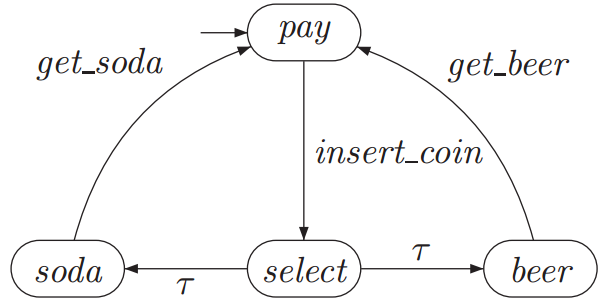
\includegraphics[scale=0.5]{images/exemplts.png}
\caption{Exemple de système à transitions étiquetées \cite{baier2008principles}}
\label{exemplts}
\end{center}
\end{figure}

La figure~\ref{exemplts} représente un système à transitions étiquetées où
\begin{itemize}
\item l'ensemble d'états est $S = (pay, select, beer, soda)$
\item les actions sont $Act = (insert\_coin, \tau, get\_soda, get\_beer)$
\item l'ensemble des transitions est $\rightarrow = (pay\xrightarrow{insert\_coin}{}select, select\xrightarrow{\tau}{}soda, select\xrightarrow{\tau}{}beer, soda\xrightarrow{get\_soda}{}pay, beer\xrightarrow{get\_beer}{}pay)$
\item L'ensemble des états initiaux est $I = (pay)$
\end{itemize}
Cet automate représente donc une machine à vendre des sodas et de la bière, en premier lieu il faut insérer une pièce, ensuite la machine sélectionne avec une probabilité d’ un demie un soda sinon une bière et le donne au client, puis finalement, retourne à l'état initial, l'état d'attente.

%On pourrait déterminer la fonction d'étiquetage comme attribuant à tout état $s$ son nom, $L(s) = \{s\}$. On pourrait aussi vouloir s'assurer que <<La machine libère la boisson seulement si elle a reçu une pièce>>, pour ce faire on définirait la fonction d'étiquetage $L$  comme :
%\begin{center}
%$L(pay) = \emptyset, L(select) = {paid}, L(soda) = L(beer) = {paid, drink}$
%\end{center}

\end{exem}

%Cet exemple montre que la sélection de la fonction d'étiquetage se fait de manière arbitraire. 
Dans l'exemple, l'action $\tau$ représente une action interne à la machine qui n'est pas utile dans sa modélisation, la transition est parfois même dépourvue d'action.\\
%Les propositions atomiques sont choisies en fonction de ce dont on souhaite prouver la propriété. Lors des représentations de ces systèmes, l'ensemble $AP$ est souvent représenté de manière non explicite, et on suppose que $AP \subseteq S$ et donc la fonction d'étiquetage est $L(s) =  \{s\} \cap AP$.\\

Dans la fin de cette sous-section, nous définissons les notions de successeurs et de prédécesseurs itérés qui permettent de représenter tous les états accessibles depuis un élément et tous les états qui ont accès à un élément.


\begin{defin}[Prédécesseur et successeur itéré\cite{baier2008principles}]
On définit $Post^*(s)$ comme étant 
\begin{center}$\underset{i \geq 0}{\cup} Post^i(s)$ avec $Post^0(s) = s$ et $Post^i(s) = Post(Post^{i-1}(s)) \forall i \geq 1$.\\
$Post^+(s)$ est $\underset{i \geq 1}{\cup} Post^i(s)$.
\end{center}
De la même façon, on définit $Pre^*(s)$ comme étant
\begin{center}
$\underset{i \geq 0}{\cup} Pre^i(s)$ avec $Pre^0(s) = s$ et $Pre^i(s) = Pre(Pre^{i-1}(s)) \forall i \geq 1$.\\
$Pre^+(s)$ est $\underset{i \geq 1}{\cup} Pre^i(s)$.
\end{center}

Ces itérations convergent vers un point fixe puisque les opérations impliquées sont monotones et que l'ensemble des états est fini.
\end{defin}

\subsection{Définition du problème}
Pour poser le problème de l'accessibilité correctement il faut encore définir ce qu'est un chemin.

\begin{defin}[Chemin \cite{geeraerts2013multiprocessor}]
Un chemin dans un automate fini $A = (V, E, S_0, F)$ est une séquence finie d'état $v_1, ..., v_t$ tel que, pour tout $1 \leq i \leq t-1 : (v_i, v_{i+1}) \in E$ 
\end{defin}

La fonction $Reach(A)$ découle de cette définition : soit $V' \subseteq V$ un ensemble d'état de $A$, s'il existe un chemin $v_1,...v_t$ dans $A$ tel que $v_t \in V'$, on dit que $v_1$ a accès à $V'$. Pour un automate $A$, on représente l'ensemble des états accessibles depuis un état initial de $A$ par la fonction $Reach(A)$.

\begin{defin}[États accessibles \cite{geeraerts2013multiprocessor}]
L'ensemble des états accessible d'un automate est défini par 
\begin{center}
$Reach(A) = \{v \in V | \exists\ un\ chemin\ v_1,...,v_t : v_1 \in S_0 \wedge v_t = v\}$
\end{center}
\end{defin}

Dès lors, le problème de l'accessibilité dans un automate pose la question de savoir si, étant donné un automate $A$ et l'ensemble d'états finaux $F$, il est possible d'accéder à un état final dans l'automate $A$, c'est à dire, de savoir si $Reach(A) \cap F = \emptyset$ ou non. On peut aussi poser la question par rapport aux prédécesseurs et successeurs itérés :

\begin{theo}[\cite{doyen2010antichain}]
Soit $A = (V,E,S_0,F)$ un automate fini, la réponse au problème de l'accessibilité de $i \in S_0$ à $F$ pour $A$ est Oui si et seulement si $Post^*(i) \cap F \neq \emptyset$ si et seulement si $\underset{f \in F}{\cup}Pre^*(f) \cap i \neq \emptyset$.
\end{theo}

La complexité en temps, soit la quantité d'opérations nécessaire pour résoudre un problème, de la fonction $Reach$ dépend du modèle utilisé. Dans le cas d'un automate fini, le problème peut se résoudre simplement par une recherche en profondeur ou en largeur, dès lors il est résoluble en temps linéaire par rapport au nombre d'états et de transitions, c'est-à-dire qu'au pire des cas, il faudra emprunter toutes les transitions et passer par tout les états. Il en va de même pour les systèmes à transitions étiquetées finis puisqu'il s'agit d'automates finis décorés.\\

Concrètement, on pourrait utiliser le problème de l'accessibilité pour vérifier qu'un programme ne peut jamais atteindre un état erroné. On créerait alors un système à transitions étiquetées $A = (V, E, S_0, F)$ avec $V$ les états du programme, $E$ les transitions du programme, $S_0$ comprenant l'état initial et $F$ l'ensemble des états erronés. On voudrait donc obtenir que $Reach(A) \cap F = \emptyset$, que $\forall i \in S_0 : Post^*(i) \cap F = \emptyset$.

\subsection{Antichaîne}
Soit un automate $A$, la fonction $Reach(A)$ est linéaire en la taille de $A$ mais il est justement possible que celle-ci soit grande. Les automates sont souvent construits pour faire un test exhaustif, comme c'est le cas en model-checking, leurs tailles deviennent alors exponentielles en le nombre de branchements du programme à vérifier, mais, bien souvent, il y a des répétitions dans ces automates fraîchement créés.\\

%\begin{exem}
%Imaginons qu'on cherche à vérifier la bonne exécution d'un programme qui aurait trois instructions indépendances entre elles, les instructions A, B et C ainsi qu'une instruction optionnelle, X. Parmi les différentes exécutions possibles, concentrons-nous sur A;B;C et A;B;C;X.\\

%On commence par vérifier que le scénario A;B;C se passe correctement et ensuite on fait de même pour le second. Lors de ces deux vérifications, la séquence A;B;C a été vérifié deux fois, alors que son comportement sera toujours le même.\\
%On va alors améliorer la performance du test en testant uniquement la séquence A;B;C;X car elle permet de tester l'autre en la simulant directement.
%\end{exem}

%Éviter de parcourir plusieurs fois les mêmes séquences d'états dans un automate généré à partir des instructions d'un logiciel permettrait de mettre en place cette optimisation.\\

Les antichaînes construisent le sous-ensemble des éléments incomparables deux à deux avec une certaine relation d'ordre (autorisant les cycles) d'un ensemble. Nous allons utiliser ces dernières avec une relation d'ordre spécifique pour qu'elles représentent des groupes d'éléments dans l'ensemble de départ. Cette relation d'ordre spécifique est une relation de simulation, cette notion et celle de l'antichaîne sont définies dans cette sous-section, en commençant le plus général, une relation d'ordre spécifique.\\

\begin{defin}[Préordres et leurs propriétés \cite{doyen2010antichain}]
Un préordre sur un ensemble fini $V$ est une relation binaire $\preceq \subseteq V \times V$ (ou $\succeq$) qui est réflexive et transitive. Si $v_1 \preceq v_2$, on dit que $v_1$ est plus petit que $v_2$ (ou que $v_2$ est plus grand que $v_1$).
Un préordre $\preceq'$ est dit plus grossier que $\preceq$ si pour tout $v_1, v_2 \in V$ si $v_1 \preceq v_2$ alors $v_1 \preceq' v_2$.\\
La $\preceq$-fermeture vers le haut d'un ensemble $S \subseteq V$ est l'ensemble $Up(\preceq, S) = \{ v_1 \in V | \exists v_2 \in S : v_2 \preceq v_1 \}$ des éléments qui sont plus grands ou égaux à un élément de $S$.
Un ensemble $S$ est $\preceq$-fermé vers le haut s'il est égal à sa $\preceq$-fermeture vers le haut, $Min(\preceq, S) = \{s_1 \in S | \forall s_2 \in S : v_2 \preceq v_1 \rightarrow v_1 \preceq v_2 \}$ reprend l'ensemble des éléments minimaux de $S$.\\
On remarque que $Min(\preceq, S) \subseteq S \subseteq Up(\preceq, S)$.\\

De la même façon, on définit la $\preceq$-fermeture vers le bas $Down(\preceq, S) = \{ v_1 \in V | \exists v_2 \in S : v_1 \preceq v_2 \}$ d'un ensemble $S$ et on dit que $S$ est $\preceq$-fermé vers le bas si $S = Down(\preceq, S)$ et $Max(\preceq, S) = \{s_1 \in S | \forall s_2 \in S : v_1 \preceq v_2 \rightarrow v_2 \preceq v_1 \}$ est l'ensemble des éléments maximaux de S.

\end{defin}

Maintenant que les préordres sont définis, nous pouvons détailler l'antichaîne se basant dessus.

\begin{defin}[Antichaîne \cite{doyen2010antichain}]
Un ensemble $H \subseteq V$ est une quasi-antichaîne si pour tout $v_1 , v_2 \in S$, soit $v_1$ et $v_2$ sont incomparable, soit $ v_1 \preceq v_2$ et $v_2 \preceq v_1$.\\
Ce même ensemble $H \subseteq V$ est une antichaîne si pour tout $v_1 , v_2 \in S$, $v_1$ et $v_2$ sont incomparable.\\
On obtient alors, une antichaîne avec la relation $\preceq$ est un sous-ensemble $H$ de $V$ tel que :
\begin{center}
$H = \{v_1 \in V|\forall v_2 \in V : v_1 \preceq v_2 \Rightarrow v_1 = v_2\}$
\end{center}

Avec un préordre, les ensembles $Min(\preceq, S)$ et $Max(\preceq, S)$ sont des quasi-antichaînes et avec un ordre partiel, un préordre antisymétrique, ces ensembles sont des antichaînes.\\
Par abus de langage, on appelle antichaîne les ensembles d'éléments minimaux ou maximaux même s'il ne s'agit pas d'un ordre partiel, mais d'un préordre.

\end{defin}

L'antichaîne nous donne les éléments incomparables d'un ensemble selon un ordre partiel. L'ordre partiel qui nous intéresse est celui de la simulation, c'est celui-là qui nous permettra de représenter plusieurs états d'un automate en un seul.

\begin{defin}[Relation de simulation \cite{doyen2010antichain}]
Soit $A = (V,E,S_0,F)$ un automate fini, on définit deux notions de simulation:
\begin{itemize}
\item un préordre $\preceq_f$ sur $V$ est une simulation vers l'avant pour $A$ si pour tout $v_1, v_2, v_3 \in V$, si $v_2 \preceq_f v_1$ et $(v_1, v_3) \in E$, alors il existe $v_4 \in V$ tel que $v_4 \preceq_f v_3$ et $(v_2, v_4) \in E$.
\item un préordre $\succeq_b$ sur $V$ est une simulation vers l'arrière pour $A$ si pour tout $v_1, v_2, v_3 \in V$, si $v_2 \succeq_b v_1$ et $(v_3, v_1) \in E$, alors il existe $v_4 \in V$ tel que $v_4 \succeq_b v_3$ et $(v_4, v_2) \in E$.
\end{itemize}
\end{defin}

Nous avons maintenant tout ce qu'il nous faut pour résoudre un problème d'accessibilité par antichaîne : l'algorithme par itérations de point fixe, les relations de simulation et les antichaînes.\\
Pour un automate $A = (V,E,S_0,F)$, une fois qu'une relation de simulation $\preceq_f$ est définie, nous sommes en mesure de créer des antichaînes $H \subseteq V$ simulant des états de l'automate $A$. On pourra alors utiliser un algorithme de points fixes qui évitera d'explorer les états représentés par une antichaîne précédemment explorée.\\

En particulier on utilisera une version modifiée de l'algorithme de point fixe $\widehat{P}ost^*(s)$ :

\begin{center}
$\underset{i\geq 0}{\cup} \widehat{P}ost^i(s)$ avec\\
$\widehat{P}ost^0(s) = Min(\preceq_f, s)$\\
$\widehat{P}ost^i(s) = Min(\preceq_f, \widehat{P}ost^{i-1}(s) \cup Post(\widehat{P}ost^{i-1}(s)))\ \forall i \geq 1$\\

\end{center}

Le développement suit la même logique dans le cas d'une simulation vers l'arrière.\\

Cette sous-section se termine en illustrant toutes ces notions avec deux exemples :

\begin{exem}[]
\begin{figure}[!h]
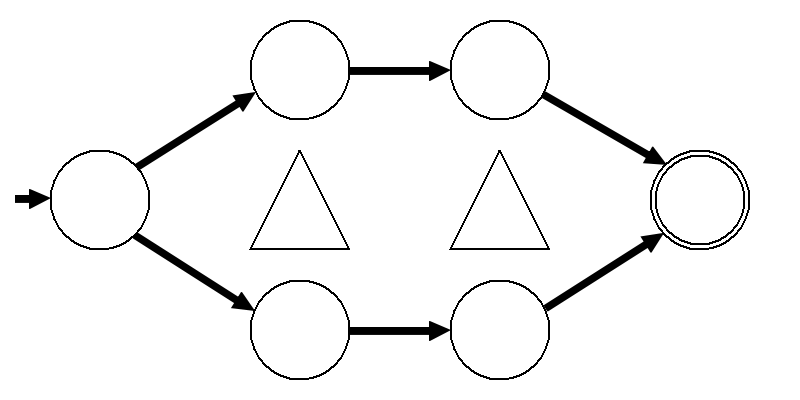
\includegraphics[width=\textwidth]{images/exanti2.png}
\caption{Exemple d'utilisation d'antichaînes}
\label{dfna}
\end{figure}

Cette illustration représente un automate fini, un cercle est un état, une flèche reliant deux cercles est une transition, l'état initial est celui avec la flèche orpheline pointant vers lui et l'état final est le double cercle.\\

Sur l'exemple en figure \ref{dfna}, on souhaite savoir s'il existe un chemin d'un état initial à un état final, nous avons identifié une relation de simulation vers l'avant $\triangleleft$, sur l'image un état avec la pointe du triangle devant lui simule celui qui a la base devant lui. Nous allons exécuter un algorithme en largeur vers l'avant. A la première itération, on obtiendra alors les deux états succédant l'initial, on utilisera la fonction $Min$ avec la relation de simulation $\triangleleft$ pour garder celui ou ceux qui ne sont simulés par aucun autre et nous continuerons à utiliser les fonctions $Post$ et $Min$ jusqu'à stabilité. Dans l'exemple, nous emprunterons donc le chemin du haut jusqu'à l'état final.

\end{exem}

Un exemple plus concret de l'utilisation de ces antichaînes se retrouve dans le cas du problème de l'universalité :

\begin{exem}[\cite{doyen2010antichain}]
Considérons la construction par sous-ensemble du complément d'un automate non déterministe (NFA) à alphabet fini. Ce complément sera un automate fini déterministe (DFA), ses états seront des groupes d'états du NFA, appelé cellule, noté $s_i$. Dans ce complément, l'inclusion entre les cellules est un ordre partiel et est une relation de simulation vers l'avant\footnote{c'est aussi une simulation vers l'arrière} : si $s_2 \subseteq s_1$ et qu'il y a une transition de $s_1$ vers $s_3$ alors il existe une transition de $s_2$ vers un $s_4 \subseteq s_3$. On retrouve cette propriété dans le problème de l'accessibilité : si $s_2 \subseteq s_1$ et une cellule finale est accessible depuis $s_1$, alors $s_2$ a accès à une cellule finale aussi. Dans ce cas, un algorithme de recherche en largeur vers l'avant pourra se permettre de ne pas explorer $s_1$ s'il explore $s_2$. En effet, $Post^*(s_1) \cap F \neq \emptyset \rightarrow Post^*(s_2) \cap F \neq \emptyset$ ce qui veut dire que si $s_2$ a accès à une cellule finale, c'est soit parce que $s_1$ y a accès soit par ce que $s_2$ possède un chemin que $s_1$ ne peut emprunter qui mène à une cellule finale. L'algorithme manipule des ensembles $\subseteq$-fermés vers le haut de cellules qui peuvent être représentés par des antichaînes de leurs éléments $\subseteq$-minimaux.\\

C'est par cette méthode que l'article \cite{doyen2010antichain} propose de résoudre le problème de l'universalité pour un NFA, avec lequel la résolution par antichaîne prend tout son sens. On aimerait savoir si un automate non déterministe accepte tous les mots de son alphabet, le but est alors de construire un DFA par sous-ensembles et d'inverser les états finaux, dès lors, si un état final est accessible par un état initial, cela signifie qu'il existe un mot qui n'est pas accepté par le NFA de base. Dans ce cadre nous pouvons utiliser la recherche en largeur vers l’avant avec antichaînes basées sur l'inclusion, une relation de simulation vers l'avant.
\end{exem}

\section{Réduction}
Ont été présentés deux problèmes qui semblent différents, de deux domaines différents de l'informatique, pourtant ils peuvent être corrélés. En effet, le but est de résoudre le problème de l'ordonnançabilité à criticité mixte en résolvant celui de l'accessibilité dans un automate. Ces deux problèmes ne sont pas liés tels quels, il va falloir réduire l'un vers l'autre, en l'occurrence, l'ordonnançabilité à criticité mixte vers le l'accessibilité dans un automate.\\

Cette réduction est une passerelle entre deux communautés des sciences informatiques qui n'ont a priori pas à se rencontrer.\\

Il s'agit donc de formaliser l'ordonnancement CM en tant que système à transitions étiquetées. La modélisation se basera sur le travail de Baker et Crinei \cite{bakerbrute}, celle-ci modélise toutes les exécutions possibles d'un système de tâche par les différents chemins possible dans un automate. Cependant, le type d'ordonnancement n'est pas le même, en effet dans le travail de Baker et Crinei on retrouve un test d'ordonnançabilité pour un système de tâche sporadique en multiprocesseur.\\

Certaines notions restent les mêmes, par exemple on se servira d'état de système, nécessitant de savoir pour chaque travail d'une instance le temps avant leur libération $nat$ et le temps restant de calcul $rct$.

\begin{defin}[État du système \cite{geeraerts2013multiprocessor}]
Étant donné une instance de $n$ travaux $I = (J_1, ..., J_n)$, l'ensemble des états du système est un ensemble de tuples $S = (nat_s, rct_s)$
\begin{itemize}
\item $nat_s$ est une fonction de $I$ vers $\mathbb{N}$ tel que pour tout $J_i : nat_s(J_i) \leq O_{max}$ avec $O_{max} = max_i\ O_i$
\item $rct_s$ est une fonction de $I$ vers $(1,...,C_{max})$ avec $C_{max} = max_i\ C_i$
\end{itemize}

Les états possibles d'une instance $I$ sont représentés par $State(I)$.\\
Ces états semblent infinis, car il n'y a pas de borne inférieure, mais il sera démontré plus tard qu'il y en a bien une.
\end{defin}

Nous remarquons ici que cette définition telle quelle n'est pas adaptée à une instance CM, car elle ne tient pas compte des différents niveaux de criticité, mais elle donne déjà une idée de l'allure qu'elle prendra. Il faudra définir les différents évènements possibles, comme un coup d'horloge ou le passage à une criticité supérieure, tout ceci se retrouvera dans le modèle.







\section{Contribution}

La première étape du mémoire sera de réduire le problème de l'ordonnancement à criticité mixte en problème d'accessibilité dans un automate. Pour ce faire, il faudra créer le modélisme qui permettra de développer tous les différents scénarios d'une instance CM selon un ordonnanceur en tant qu'automate fini.\\

Ensuite, il faudra transformer les états de cet automate en antichaînes dans le but de réduire le temps de parcours du graphe, il faudra donc définir la relation de simulation pour les différents états en tenant compte des contraintes posées par la criticité mixte.\\

Une fois la modélisation terminée, une implémentation logicielle du problème sera mise en place dans le but de tester l'efficacité de la résolution du problème de certification. Ceci sera accompagné de comparatifs entre la méthode de résolution avec antichaînes et sans.


\chapter{Test d'ordonnancement}
\section{Tache Périodique}
\subsection{Modèle sous forme d'automate}

Le but de cette section est de modéliser les différentes exécutions d'un ensemble de tâches en criticité mixte ordonnancé par un algorithme donné sous la forme d'un automate fini.\\

\begin{defin}[État du système]
Soit $\tau = \tau_1, \tau_2, \tau_3 ...$ un ensemble de tâches périodiques en criticité mixte, l'état du système de $\tau$ est le tuple $S = (at_S, rct_S, crit_S)$ avec

\begin{itemize}
\item $at_S$, une fonction représentant le temps d'arrivée du travail courant d'une tâche : $\tau \rightarrow \mathbb{N},\ at_S(\tau_i) \leq R_{max}$ avec $R_{max} = max(max_i\ (T_i),\ max_i\ (O_i))$
\item $rct_S$, le temps de calcul restant du travail généré par une tâche : $ \tau \rightarrow \mathbb{N},\ 0 \leq rct_S(\tau_i) \leq C_{max}$ avec $C_{max} = max_{i,j}\ C_i(j)$
\item $crit_S$, le niveau de criticité actuel du scénario, $ \in \mathbb{N},\ 0 \leq crit_S \leq K$

\end{itemize}

\end{defin}

Pour définir les transitions de l'automate, il faut définir des notions auxiliaires.

\begin{defin}[Tâches actives et disqualifiées]
Une tâche est active dans l'état $S$ si elle est arrivée dans celui-ci et n'est pas disqualifiée.

$Active(S) = \{\tau_i | at_S(\tau_i) < 0\vee (at_S(\tau_i) == 0 \wedge rct_S(\tau_i) > 0)\}$\\

Une tâche est dite disqualifiée lors ce que sa criticité est inférieure à celle de l'état. Ces tâches sont représentées dans le système comme ayant un temps de calcul restant et le temps d'arrivée nul.

$Discarded(S) = \{\tau_i | at_S(\tau_i) == 0 \wedge rct_S(\tau_i) == 0\}$
\end{defin}


\begin{defin}[Tâche implicitement terminée]
Dans le modèle, ce sont les tâches elles-mêmes qui signalent la complétion de leurs travaux. En revanche il existe un cas où les travaux seront implicitement finis : celui où le système est au niveau de la criticité du travail et que le travail a été exécuté complètement.\\
Cette transition vient du fait que, dans le modèle, un travail n'excède pas son WCET maximal.

$ImplicitelyDone(S) = \{\tau_i | rct_S == 0 \wedge\ at_S(\tau_i) < 0\wedge crit_S=\chi_i\}$\\
\end{defin}


\begin{defin}[Criticité d'un état]
La criticité réelle d'un état $S$ est celle de l'état si aucune tâche n'a été exécutée complètement sans avoir signalé sa complétion, celle de l'état incrémentée d'un sinon.
$$
Critical_S = \left\{
    \begin{array}{ll}
        crit_S+1 & \exists \tau_i \in Active(S)\ tq\ rct_S(\tau_i) == 0 \\
        crit_S & \mbox{sinon.}
    \end{array}
\right.
$$
\end{defin}

\begin{defin}[Laxité]
La laxité d'une tâche $\tau_i$ d'un état $S$ est :

$Laxity_S(\tau_i) = at_S(\tau_i)  + D_i - rct_S(\tau_i))$\\

La laxité d'une tâche est donc le nombre d'unités de temps où la tâche peut être oisive avant de manquer son échéance. Dès lors, si la laxité d'une des tâches d'un état est négative, une tâche manquera son échéance. Cette définition permet de donner celle des états erronés.
\end{defin}

\begin{defin}[États erronés]
Un état $S$ est erroné si l'une des laxités des tâches est négative, on obtient alors l'ensemble :

$Fail_\tau = \{S|\exists \tau_i \in \tau : Laxity_S(\tau_i) < 0  \}$\\
\end{defin}

Grâce à ces états erronés, nous pouvons à présent borner inférieurement $at_S$. En effet, puisque dès que la laxité d'un état est négative, il est érroné, il n'est pas nécéssaire d'inclure dans l'automate les état où $\exists\ \tau_i \in \tau\ tq\ Laxity_S(\tau_i) < -1$. Dés lors : $at_S(\tau_i) + D_{max} - rct_S(\tau_i) \geq -1$ d'où $at_S(\tau_i) \geq rct_S(\tau_i) - (D_{max}+1) \geq -(D_{max}+1)$ et donc $-(D_{max}+1) \leq at_S(\tau_i) \leq R_{max}$ avec $D_{max} = max_i\ D_i$ et $R_{max} = max(max_i\ (T_i),\ max_i\ (O_i))$\\

Nous pouvons à présent définir les transitions de l'automate. Pour ce faire nous devons choisir un $ordonnanceur$, une fonction sur un état vers une tâche à ordonnancer.

\begin{defin}[Ordonnanceur]
Un $ordonnanceur$ monoprocesseur pour $\tau$ est une fonction $Run : State(\tau) \rightarrow \tau$ telle que $Run(S) \subseteq Active(S)$ et $0 \leq |Run(S)| \leq 1$.
De plus :
\begin{itemize}
\item $Run$ est $work-conserving$ ssi pour $S$ : $ |Run(S)| = min\{1, |Exectuable(S)|\}$
\item $Run$ est $sans\ memoire$ ssi pour $S_1,S_2$ avec $Active(S_1) == Active(S_2)$:
$\forall \tau_i \in Active(S_1) : (at_{S_1} == at_{S_2} \wedge rct_{S_1} == rct_{S_2} \wedge crit_{S_1} == crit_{S_2} )$ implique $Run(S_1) == Run(S_2)$
\end{itemize}

\end{defin}

\begin{defin}[Transition d'exécution]
Soit $S = (at_S, rct_S, crit_S)$ un état du système et $Run$ un $ordonnanceur$ pour $\tau$. On dit que l'état du système $S^+ = (at_S^+, rct_S^+, crit_S^+)$ est un $successeur\ horloge$ de $S$ avec $Run$, noté $S\xrightarrow{Run}S^+$ ssi:
\begin{itemize}
\item Pour tout $\tau_i \in Run(S) : rct_S^+(\tau_i) = rct_S(\tau_i)-1$\\
\item Pour tout $\tau_i \not \in Run(S) : rct_S^+(\tau_i) = rct_S(\tau_i)$\\
\item Pour tout $\tau_i \in \tau :$
$$ at_S^+(\tau_i) = \left\{
    \begin{array}{ll}
        0 & si\ \chi_i < crit_S \\
        at_S(\tau_i)-1 & si\ \chi_i \geq crit_S \\
    \end{array}
\right.
$$\\
\item $crit_{S}^{+} = crit_{S}$

\end{itemize}
Cette transition permet à une tâche de profiter de la ressource partagée pendant un coup d'horloge, ce qui signifie que la tâche ordonnancée verra son temps restant d'exécution décrémentée d'une unité et le temps d'arrivé de toutes les tâches sera lui aussi décrémenté d'une unité, sauf pour les tâches qui ne sont plus considérées de par la criticité de l'état du système.
\end{defin}

\begin{defin}[Transition de terminaison]
Soit $S = (at_S, rct_S, crit_S)$ un état du système et $\tau' \subseteq Active(S)$ un ensemble de tâches actives pouvant signaler leur complétion. On dit que l'état du système $S' = (at_S', rct_S', crit_S')$ est un $successeur\ \tau'-terminaison$ de $S$, noté $S\xrightarrow{\tau'}S'$ ssi:
\begin{itemize}
\item Pour tout $\tau_i \in \tau' \cup ImplicitelyDone(S)$ :\begin{itemize}
\item $rct_{S'}(\tau_i) = C_i(crit_S)$
\item $at_{S'}(\tau_i) = at_{S}(\tau_i)+T_i$
\end{itemize}

\item Pour tout $\tau_i\ not\ \in \tau' \cup ImplicitelyDone(S)$ :\begin{itemize}
\item $rct_{S'}(\tau_i) = rct_{S}(\tau_i)$
\item $at_{S'}(\tau_i) = at_{S}(\tau_i)$
\end{itemize}
\item $crit_{S'} = crit_{S}$

\end{itemize}
Cette transition représente les complétions signalée ou implicite de travaux de tâches.
\end{defin}

\begin{defin}[Transition critique]
Soit $S = (at_S, rct_S, crit_S)$ un état du système. On dit que l'état du système $S^C = (at_S^C, rct_S^C, crit_S^C)$ est un $successeur\ critique$ de $S$, noté $S\xrightarrow{C}S^C$, ssi :
\begin{itemize}
\item $crit_S^C = Critical_S$
\item Pour tout $\tau_i \in \tau :$
$$ rct_S^C(\tau_i) = \left\{
    \begin{array}{ll}
        rct_S+c_i(Critical_S)-c_i(crit_S) & si\ X_i\geq Critical_S \\
        0 & \mbox{sinon.}
    \end{array}
\right.
$$
$$ at_S^C(\tau_i) = \left\{
    \begin{array}{ll}
        at_S & si\ X_i\geq Critical_S \\
        0 & \mbox{sinon.}
    \end{array}
\right.
$$\\
\end{itemize}
Cette transition met à jour la criticité du système et augmente les temps restants d'exécution si nécessaire. Si la criticité dépasse celle de certaines tâches, leur temps d'arrivé et leur temps d'exécution sont mis à zéro et rejoigne donc bien l'ensemble $Discarded(S^C)$.
\end{defin}

\begin{defin} Étant donné un ensemble de tâches $\tau$ et un ordonnanceur $Run$, l'automate $A(\tau,Run)$ est le tuple $(V, E, S_0, F)$ où:
\begin{itemize}
\item  $V=State(\tau)$
\item $(S_1,S_2) \in E$ ssi il existe les états intermédiaires $S'$ et $S'' \in State(\tau)$ et $\tau' \subseteq Active(S') $ tel que : $S_1\xrightarrow{Run}S'\xrightarrow{\tau'}S''\xrightarrow{C}S_2$
\item $S_0 = (at_{S_0}, rct_{S_0}, crit_{S_0})$ :\begin{itemize}
\item $at_{S_0} = O_i\ \forall \tau_i \in \tau$
\item $rct_{S_0} = C_i(1)\ \forall \tau_i \in \tau$
\item $crit_{S_0} = 1$
\end{itemize}
\item $F = Fail_\tau$
\end{itemize}

\end{defin} 


\section{Tâche Sporadique}
\subsection{Modèle sous forme d'automate}


\begin{defin}[État du système]
\label{systemstate}
Soit $\tau = \tau_1, \tau_2, \tau_3 ...$ un ensemble de tâches périodiques en criticité mixte, l'état du système de $\tau$ est le tuple $S = (nat_S, rct_S, done_S, crit_S)$ avec

\begin{itemize}
\item $nat_S$, une fonction représentant le temps d'arrivée du prochain travail d'une tâche au plus tôt : $\tau \rightarrow \mathbb{N},\ at_S(\tau_i) \leq R_{max}$ avec $R_{max} = max(max_i\ (T_i),\ max_i\ (O_i))$
\item $rct_S$, le temps de calcul restant du travail généré par une tâche : $ \tau \rightarrow \mathbb{N},\ 0 \leq rct_S(\tau_i) \leq C_{max}$ avec $C_{max} = max_{i,j}\ C_i(j)$
\item $done_S$, la complétion d'un travail : $ \tau \rightarrow \{0,1\}$
\item $crit_S$, le niveau de criticité actuel du scénario, $ \in \mathbb{N},\ 0 \leq crit_S \leq K$

\end{itemize}

\end{defin}

\begin{defin}[Tâches actives]
\label{active}
$Active(S) = \{\tau_i | !done_S(\tau_i)\}$
\end{defin}


\begin{defin}[Tâche implicitement terminée]
\label{impdone}

$ImplicitelyDone(S) = \{\tau_i | rct_S(\tau_i) == 0 \wedge\ !done_S(\tau_i)\wedge crit_S=\chi_i\}$\\
\end{defin}


\begin{defin}[Tâche éligible à la submission d'un travail]
\label{eligible}
$Eligibile(S) = \{\tau_i | rct_S(\tau_i) == 0 \wedge\ nat_S(\tau_i) \leq 0 \wedge\ done_S(\tau_i)\wedge\ crit_S\geq\chi_i\}$\\
\end{defin}


\begin{defin}[Criticité d'un état]
\label{critical}
La criticité réelle d'un état $S$ est celle de l'état si aucune tâche n'a été exécutée complètement sans avoir signalé sa complétion, celle de l'état incrémentée d'un sinon.
$$
Critical_S = \left\{
    \begin{array}{ll}
        crit_S+1 & \exists \tau_i \in Active(S)\ tq\ rct_S(\tau_i) == 0 \\
        crit_S & \mbox{sinon.}
    \end{array}
\right.
$$
\end{defin}

\begin{defin}[Laxité]
\label{laxity}
La laxité d'une tâche $\tau_i$ dans l'état $S$ est :

$Laxity_S(\tau_i) = nat_S(\tau_i) -T_i + D_i - rct_S(\tau_i)$\\

La laxité d'une tâche est donc le nombre d'unités de temps où la tâche peut être oisive avant de manquer son échéance. Dès lors, si la laxité d'une des tâches d'un état est négative, une tâche manquera son échéance. Cette définition permet de donner celle des états erronés.
\end{defin}

\begin{defin}[États erronés]
\label{failstate}
Un état $S$ est erroné si l'une des laxités des tâches est négative, on obtient alors l'ensemble :

$Fail_\tau = \{S|\exists \tau_i \in \tau : Laxity_S(\tau_i) < 0  \}$\\
\end{defin}

Grâce à ces états erronés, nous pouvons à présent borner inférieurement $at_S$. En effet, puisque dès que la laxité d'un état est négative, il est érroné, il n'est pas nécéssaire d'inclure dans l'automate les état où $\exists\ \tau_i \in \tau\ tq\ Laxity_S(\tau_i) < -1$.\\
Dés lors : $nat_S(\tau_i) -T_{min} + D_{max} - rct_S(\tau_i) \geq -1$\\
d'où $nat_S(\tau_i) \geq rct_S(\tau_i) - (D_{max}+1) + T_{min} \geq T_{min}-(D_{max}+1)$\\
et donc $T_{min}-(D_{max}+1) \leq nat_S(\tau_i) \leq R_{max}$\\
avec $D_{max} = max_i\ D_i$ et $R_{max} = max(max_i\ (T_i),\ max_i\ (O_i))$\\

Nous pouvons à présent définir les transitions de l'automate. Pour ce faire nous devons choisir un $ordonnanceur$, une fonction sur un état vers une tâche à ordonnancer.

\begin{defin}[Ordonnanceur]
\label{run}
Un $ordonnanceur$ monoprocesseur pour $\tau$ est une fonction $Run : State(\tau) \rightarrow \tau$ telle que $Run(S) \subseteq Active(S)$ et $0 \leq |Run(S)| \leq 1$.
De plus :
\begin{itemize}
\item $Run$ est $work-conserving$ ssi pour $S$ : $ |Run(S)| = min\{1, |Exectuable(S)|\}$
\item $Run$ est $sans\ memoire$ ssi pour $S_1,S_2$ avec $Active(S_1) == Active(S_2)$:
$\forall \tau_i \in Active(S_1) : (nat_{S_1} == nat_{S_2} \wedge rct_{S_1} == rct_{S_2} done_{S_1} == done_{S_2} \wedge crit_{S_1} == crit_{S_2} )$ implique $Run(S_1) == Run(S_2)$
\end{itemize}

\end{defin}

\begin{defin}[Transition d'exécution]
\label{texec}
Soit $S = (nat_S, rct_S, done_S, crit_S)$ un état du système et $Run$ un $ordonnanceur$ pour $\tau$. On dit que l'état du système $S^+ = (nat_S^+, rct_S^+, done_S^+, crit_S^+)$ est un $successeur\ horloge$ de $S$ avec $Run$, noté $S\xrightarrow{Run}S^+$ ssi:
\begin{itemize}
\item Pour tout $\tau_i \in Run(S) : rct_S^+(\tau_i) = rct_S(\tau_i)-1$\\
\item Pour tout $\tau_i \not \in Run(S) : rct_S^+(\tau_i) = rct_S(\tau_i)$\\
\item Pour tout $\tau_i \in \tau :$
$$ nat_S^+(\tau_i) = \left\{
    \begin{array}{ll}
        max(nat_S(\tau_i)-1, 0) & si\ done_S(\tau_i) \\
        nat_S(\tau_i)-1 & si\ !done_S(\tau_i) \\
    \end{array}
\right.
$$
\begin{center}
$done_{S}^{+}(\tau_i) = done_{S}(\tau_i)$

\end{center}
\item $crit_{S}^{+} = crit_{S}$

\end{itemize}
Cette transition permet à une tâche de profiter de la ressource partagée pendant un coup d'horloge, ce qui signifie que la tâche ordonnancée verra son temps restant d'exécution décrémentée d'une unité et le temps d'arrivé de toutes les tâches sera lui aussi décrémenté d'une unité, sauf pour les tâches qui ne sont plus considérées de par la criticité de l'état du système.
\end{defin}

\begin{defin}[Transition de terminaison]
\label{tterm}
Soit $S = (nat_S, rct_S, done_S, crit_S)$ un état du système et $\tau^T \subseteq Run(S)$ un ensemble de tâches actives pouvant signaler leur complétion. On dit que l'état du système $S^T = (nat_S^T, rct_S^T, done_S^T, crit_S^T)$ est un $successeur\ \tau^T-terminaison$ de $S$, noté $S\xrightarrow{\tau^T}S^T$ ssi:
\begin{itemize}
\item Pour tout $\tau_i \in \tau^T \cup ImplicitelyDone(S)$ :\begin{itemize}
\item $rct_{S}^T(\tau_i) = 0$
\item $nat_{S}^T(\tau_i) = nat_{S}(\tau_i)$
\item $done_{S}^T(\tau_i) = True$
\end{itemize}

\item Pour tout $\tau_i\ not\ \in \tau^T \cup ImplicitelyDone(S)$ :\begin{itemize}
\item $rct_{S}^T(\tau_i) = rct_{S}(\tau_i)$
\item $nat_{S}^T(\tau_i) = nat_{S}(\tau_i)$
\item $done_{S}^T(\tau_i) = done_{S}(\tau_i)$
\end{itemize}
\item $crit_{S}^T = crit_{S}$

\end{itemize}
Cette transition représente les complétions signalée ou implicite de travaux de tâches.

Pour un état $S$, on note l'ensemble de ses $successeur\ \tau^T-terminaison$ $S^{\tau^T}$
\end{defin}

\begin{defin}[Transition critique]
\label{tcrit}
Soit $S = (at_S, rct_S, done_S, crit_S)$ un état du système. On dit que l'état du système $S^C = (at_S^C, rct_S^C, done_S^C, crit_S^C)$ est un $successeur\ critique$ de $S$, noté $S\xrightarrow{C}S^C$, ssi :
\begin{itemize}
\item $crit_S^C = Critical_S$
\item Pour tout $\tau_i \in \tau :$
$$ rct_S^C(\tau_i) = \left\{
    \begin{array}{ll}
        rct_S(\tau_i)+c_i(Critical_S)-c_i(crit_S) & si\ X_i\geq Critical_S \\
        0 & \mbox{sinon.}
    \end{array}
\right.
$$
$$ nat_S^C(\tau_i) = \left\{
    \begin{array}{ll}
        nat_S(\tau_i) & si\ X_i\geq Critical_S \\
        0 & \mbox{sinon.}
    \end{array}
\right.
$$
$$ done_S^C(\tau_i) = \left\{
    \begin{array}{ll}
        done_S(\tau_i) & si\ X_i\geq Critical_S \\
        True & \mbox{sinon.}
    \end{array}
\right.
$$\\
\end{itemize}
Cette transition met à jour la criticité du système et augmente les temps restants d'exécution si nécessaire. Si la criticité dépasse celle de certaines tâches, leur temps d'arrivé et leur temps d'exécution sont mis à zéro et rejoigne donc bien l'ensemble $Discarded(S^C)$.
\end{defin}


\begin{defin}[Transition de requête]
\label{treq}
Soit $S = (nat_S, rct_S, done_S, crit_S)$ un état du système et $\tau^R \subseteq Eligible(S)$ un ensemble de tâches eligible. On dit que l'état du système $S^R = (nat_S^R, rct_S^R, done_S^R, crit_S^R)$ est un $successeur\ \tau^R-request$ de $S$, noté $S\xrightarrow{\tau^R}S^R$ ssi:

\begin{itemize}
\item Pour tout $\tau_i \in \tau^R$ :\begin{itemize}
    \item $nat_S(\tau_i)+T_i \leq nat_S^R(\tau_i) \leq T_i$
    \item $rct_S^R(\tau_i)=C_i(crit_S)$
    \item $done_S^R(\tau_i) = False$
\end{itemize}
\item Pour tout $\tau_i\ not \in \tau^R$ :\begin{itemize}
    \item $nat_S^R(\tau_i)=nat_S(\tau_i)$
    \item $rct_S^R(\tau_i)=rct_S(\tau_i)$
    \item $done_S^R(\tau_i) = done_S(\tau_i)$
\end{itemize}
\item $crit_S^R = crit_S$
\end{itemize}

Pour un état $S$, on note l'ensemble de ses $successeur\ \tau^R-request$ $S^{\tau^R}$

\end{defin}

\begin{defin} 
\label{autospo}
Étant donné un ensemble de tâches $\tau$ et un ordonnanceur $Run$, l'automate $A(\tau,Run)$ est le tuple $(V, E, S_0, F)$ où:
\begin{itemize}
\item  $V=State(\tau)$
\item $(S_1,S_2) \in E$ ssi il existe les états intermédiaires $S^{+}, S^{T}$ et $S^{C} \in State(\tau)$ et $\tau^T \subseteq Active(S^{+}),\tau^R \subseteq Eligilbe(S^{T}) $ tel que : \\$S_1\xrightarrow{Run}S^{+}\xrightarrow{\tau^T}S^{T}\xrightarrow{C}S^{C}\xrightarrow{\tau^R}S_2$
\item $S_0 = (nat_{S_0}, rct_{S_0}, done_{S_0}, crit_{S_0})$ :\begin{itemize}
\item $nat_{S_0}(\tau_i) = 0\ \forall \tau_i \in \tau$
\item $rct_{S_0}(\tau_i) = 0\ \forall \tau_i \in \tau$
\item $done_{S_0}(\tau_i) = True\ \forall \tau_i \in \tau$
\item $crit_{S_0} = 1$
\end{itemize}
\item $F = Fail_\tau$
\end{itemize}

\end{defin} 

\subsection{Antichaine}

\subsubsection{Simulation de tâche oisive}

\begin{defin}[Simulation de tâche oisive]
\label{idlesim}
Soit $\tau$ un ensemble de tâche sporadique de criticité mixte. Le préordre de tâche oisive $\succeq_{idle} \subseteq State(\tau)\times State(\tau)$ est tel que pour tout $S_1, S_2 : S_1 \succeq_{idle}S_2$ ssi:
\begin{itemize}
\item $crit_{S_1} = crit_{S_2}$
\item $done_{S_1} = done_{S_2}$
\item $rct_{S_1} = rct_{S_2}$
\item Pour tout $\tau_i$ tel que $done_{S_1} : nat_{S_1} \leq nat_{S_2}$
\item Pour tout $\tau_i$ tel que $!done_{S_1} : nat_{S_1} = nat_{S_2}$
\end{itemize}
Cette relation est transitive et réflexive, il s'agit donc bien d'un préordre. La relation défini aussi un ordre partiel sur $Active(S)$ car celle ci est anti-symétrique.
Remarquons que $Active(S_1) = Active (S_2)$ puisque $done_{S_1} = done_{S_2}$
\end{defin}

\begin{lem}
\label{runeq}
Si $S_1$ et $S_2$ sont est états tel que $S_1 \succeq_{idle}S_2$ et $Run$ un ordonnanceur sans mémoire alors $Run (S_1) = Run(S_2)$.
\end{lem}
\begin{proof} Par \autoref{idlesim}: $S_2 \succeq_{idle} S_1$ implique que $Active(S_1) = Active(S_2)$. Soit $\tau_i$ un tâche faisant partie de $Active(S_1)$, d'où $done_{S_1}(\tau_i) = False$. Dans ce cas, et puisque $S_2 \succeq_{idle} S_1$, on en conclu que $done_{S_1}(\tau_i) = done_{S_2}(\tau_i)$, $nat_{S_1}(\tau_i) = nat_{S_1}(\tau_i)$, $rct_{S_1}(\tau_i) = rct_{S_1}(\tau_i)$ et que $crit_{S_1} = crit_{S_2}$ pour tout $\tau_i \in Active(S_1)$. Donc, comme $Run$ est sans mémoire par hypothèse, $Run(S_1) = Run(S_2)$.
\end{proof}

\begin{lem}
\label{impdoneeq}
Si $S_1$ et $S_2$ sont est états tel que $S_1 \succeq_{idle}S_2$ alors $ImplicitelyDone(S_1) = ImplicitelyDone(S_2)$.
\end{lem}
\begin{proof} Par \autoref{idlesim}: $S_2 \succeq_{idle} S_1$ implique que $done_{S_1}(\tau_i) = done_{S_2}(\tau_i)$, $rct_{S_1}(\tau_i) = rct_{S_1}(\tau_i)$ et que $crit_{S_1} = crit_{S_2}$ pour tout $\tau_i \in \tau$. D'où $ImplicitelyDone(S_1) = ImplicitelyDone(S_2)$.
\end{proof}

\begin{lem}
\label{criteq}
Si $S_1$ et $S_2$ sont est états tel que $S_1 \succeq_{idle} S_2$ alors $Critical_{S_1} = Critical_{S_2}$.
\end{lem}
\begin{proof} Par \autoref{idlesim}: $S_2 \succeq_{idle} S_1$ implique que $Active(S_1) = Active(S_2)$, $crit_{S_1} = crit_{S_2}$ et que $rct_{S_1}(\tau_i) = rct_{S_1}(\tau_i)$ pour tout $\tau_i \in \tau$. D'où $Critical_{S_1} = Critical_{S_2}$.
\end{proof}





\begin{lem}
\label{elisuper}
Si $S_1$ et $S_2$ sont deux états tel que $S_1 \succeq_{idle}S_2$ alors $Eligible(S_1) \supseteq Eligible(S_2)$.
\end{lem}
\begin{proof} Prouvons que toute tâche $\tau_i \in Eligible(S_2) \rightarrow \tau_i \in Eligible(S_1)$. Puisque $\tau_i \in Eligible(S_2)$, on a $done_{S_2}(\tau_i) = True$,  $crit_{S_2} \leq \chi_i$, et $nat_{S_2}(\tau_i) \leq 0$ par définition de $Eligible$. Donc, puisque $S_1 \succeq_{idle}S_2$, $done_{S_1}(\tau_i) = done_{S_2}(\tau_i) = True$,  $crit_{S_1} = crit_{S_2} \leq \chi_i$ et $nat_{S_1}(\tau_i) \leq nat_{S_2}(\tau_i) \leq 0$ par définition de $\succeq_{idle}$. D'où $\tau_i \in Eligible(S_1)$.
\end{proof}

\begin{defin}
\label{reqanalogue}
Soit $S_1$ et $S_2$ deux états tel que $S_1 \succeq_{idle}S_2$ et $\tau^R \subseteq Eligible(S_2)$. Alors, pour tout $\overline{S}_2\in S_2^{\tau^R}$, un état  $\overline{S}_1\in S_1^{\tau^R}$ est appelé $analogue\ \tau^R-oisif$ de $\overline{S}_2$ ssi:
\begin{center}
$\forall \tau_i \in \tau^R : nat_{\overline{S}_1}(\tau_i) = nat_{\overline{S}_2}(\tau_i) $
\end{center}
\end{defin}

\begin{lem}
\label{reqanalogueeq}
Soit $S_1$ et $S_2$ deux états tel que $S_1 \succeq_{idle} S_2$ et $\tau^R \subseteq Eligible(S_2)$ un sous-ensemble de tache. Alors, pour tout $\overline{S}_2 \in S_2^{\tau^R}$ il y a un $analogue\ \tau^R-oisif\ \overline{S}_1 \in S_1^{\tau^R}$ de $\overline{S}_2$.
\end{lem}
\begin{proof}
\autoref{treq} et \autoref{idlesim} pose que pour tout $\tau_i \in \tau^R \subseteq Eligible(S_2)$ on a $nat_{S_1}(\tau_i) \leq nat_{S_2}(\tau_i) \leq 0$, $rct_{S_1}(\tau_i) = rct_{S_2}(\tau_i) = 0$, $done_{S_1}(\tau_i) = done_{S_2}(\tau_i) = True$ et que $crit_{S_1} = crit_{S_2}$. Par définition, tout $\overline{S}_2 \in S^{\tau^R}_2$ satisfait :
\begin{center}
$\forall \tau_i \in \tau^R : nat_{\overline{S}_2}(\tau_i) \in I^i_2=[nat_{S_2}(\tau_i)+T_i, T_i] $
\end{center}
De manière similaire, par définition $X$, pour tout vecteur $(k_1, k_2, ..., k_n)(ou\ n = |\tau^R|)$ tel que pour tout $1\leq i \leq n: k_i \in I^i_1=[nat_{S_1}(\tau_i)+T_i, T_i]$, il existe $\overline{S}_1\in S^{\tau^R}_1$ avec $nat_{\overline{S}_1}(\tau_i) = k_i$ pour tout $1\leq i \leq n$. C'est à dire qu'à chaque fois qu'un vecteur $(k_1, k_2, ..., k_n)$ de valeurs dans $I_1^1 \times I_1^2 \times ... \times I_1^n$ est fixé, il est possible de trouver un état $\overline{S}_1 \in S^{\tau^R}_1$ tel que le $nat$ de chaque tâche $\tau_i$ est exactement $k_i$. Cependant, comme $nat_{S_1}(\tau_i) \leq nat_{S_2}(\tau_i)$ pour tout $1\leq i \leq n$ on en conclu que $nat_{S_2}(\tau_i) \in I^i_2 \subseteq I^i_1$ pour tout $1\leq i \leq n$. Dés lors, le vecteur $nat_{\overline{S}_2}(\tau_1), nat_{\overline{S}_2}(\tau_2), ..., nat_{\overline{S}_2}(\tau_n)$ est dans $I_1^1 \times I_1^2 \times ... \times I_1^n$. D'où il existe $\overline{S}_1 \in S^{\tau^R}_1$ tel que pour tout $1\leq i \leq n : nat_{\overline{S}_1}(\tau_i) = nat_{\overline{S}_2}(\tau_i)$
\end{proof}


Prouvons maintenant que $\succeq_{idle}$ est bien une relation de simulation lors ce qu'on considère un ordonnanceur sans mémoire.

\begin{theo}
Soit $\tau$ un ensemble de tâche sporadique à mixité critique and $Run$ un ordonnanceur sans mémoire (déterminé) pour $\tau$ sur un processeur. Alors, $\succeq_{idle}$ est une relation de simulation pour $A(\tau, Run)$.
\end{theo}

\begin{proof}
Soit $S_1, S'_1$ et $S_2$ trois état dans $States(\tau)$ tel que $(S_1, S_1') \in E$ et $S_2 \succeq_{idle}S_1$, montrons qu'il existe $S_2' \in States(\tau)$ avec $(S_2, S_2') \in E$ and $S_2' \succeq_{idle} S_1'$.\\

Puisque $(S_1, S_1') \in E$, il existe $S^{+}_1, S^{T}_1$ et $S^{C}_1 \in State(\tau)$ et $\tau^T \subseteq Active(S^{+}_1),\tau^R \subseteq Eligilbe(S^{T}_1) $ tel que : $S_1\xrightarrow{Run}S^{+}_1\xrightarrow{\tau^T}S^{T}_1\xrightarrow{C}S^{C}_1\xrightarrow{\tau^R}S_1'$.\\

Par \autoref{idlesim}, $S_2 \succeq_{idle} S_1$ implique que $Active(S_1) = Active(S_2)$. Soit $\tau_i$ un tâche faisant partie de $Active(S_1)$, d'où $done_{S_1}(\tau_i) = False$. Dans ce cas, et puisque $S_2 \succeq_{idle} S_1$, on en conclu que $done_{S_1}(\tau_i) = done_{S_2}(\tau_i)$, $nat_{S_1}(\tau_i) = nat_{S_1}(\tau_i)$, $rct_{S_1}(\tau_i) = rct_{S_1}(\tau_i)$ et que $crit_{S_1} = crit_{S_2}$ pour tout $\tau_i \in Active(S_1)$. Donc, comme $Run$ est sans mémoire par hypothèse, $Run(S_1) = Run(S_2)$. Soit $S^+_1$ l'état unique tel que $S_1\xrightarrow{Run}S^{+}_1$, montrons qu'il existe $S^+_2$ tel que $S_2\xrightarrow{Run}S^{+}_2$ et que $S^+_2 \succeq_{idle} S^+_1$.
\begin{enumerate}

\item Pour tout $\tau_i \in Run(S_1) = Run(S_2) : rct_{S_1}^+(\tau_i) = rct_{S_1}(\tau_i) -1, rct_{S_2}^+(\tau_i) = rct_{S_2}(\tau_i) -1$. Puisque $S_2 \succeq_{idle} S_1$, on sait que $rct_{S_1} = rct_{S_2}$. D'où $rct_{S_2}^+(\tau_i) = rct_{S_1}^+(\tau_i)$. Pour une tâche $\tau_1 \notin Run(S_1) = Run(S_2) : rct_1^+(\tau_i) = rct_1(\tau_i), rct_2^+(\tau_i) = rct_2(\tau_i)$. D'où $rct_{S_2}^+(\tau_i) = rct_{S_1}^+(\tau_i)$. On en conclut alors que $rct_{S_2}^+ = rct_{S_1}^+$.


\item Pour tout  $\tau_i \in \tau : done_{S_1}^+(\tau_i) = done_{S_1}(\tau_i), done_{S_2}^+(\tau_i) = done_{S_2}(\tau_i)$. Puisque $S_2 \succeq_{idle} S_1$, on a aussi que $done_{S_1}(\tau_i) = done_{S_2}(\tau_i)$. On en conclu que $done_{S_1}^+ = done_{S_2}^+$.

\item $crit_{S_1}^+ = crit_{S_1}, crit_{S_2}^+ = crit_{S_2}$. Puisque $S_2 \succeq_{idle} S_1$, on a aussi que $crit_{S_1} = crit_{S_2}$. On en conclu que $crit_{S_1}^+ = crit_{S_2}^+$.

\item Soit $\tau_i$ un tâche tel que $done_{S_1}^+(\tau_i) = True : nat_{S_1}^+ = max(nat_{S_1}(\tau_i)-1, 0)$ et $nat_{S_2}^+ = max(nat_{S_2}(\tau_i)-1, 0)$. Cependant, comme $S_2 \succeq_{idle} S_1$, on sait que $nat_{S_2} \leq nat_{S_1}$. On en conclu que $nat_{S_2}^+ \leq nat_{S_1}^+$.

\item Soit $\tau_i$ un tâche tel que $done_{S_1}^+(\tau_i) = False : nat_{S_1}^+ = nat_{S_1}(\tau_i)-1$ et $nat_{S_2}^+ = nat_{S_2}(\tau_i)-1$. Cependant, comme $S_2 \succeq_{idle} S_1$, on sait que $nat_{S_2} \leq nat_{S_1}$. On en conclu que $nat_{S_2}^+ \leq nat_{S_1}^+$. Comme $done_{S_1}^+(\tau_i) = False$, $done_{S_1}(\tau_i) = False$ aussi car une tâche ne peut signaler sa complétion qu'après une exécution. Puisque $S_2 \succeq_{idle} S_1$, on a aussi que $nat_{S_2}(\tau_i) = nat_{S_1}(\tau_i)$. On en conclu que $nat_{S_2}^+(\tau_i) = nat_{S_1}^+(\tau_i)$.
\end{enumerate}
Par \autoref{texec}. Il est maintenant établi que $S^+_2 \succeq_{idle} S^+_1$.\\

Par le \autoref{runeq} et le \autoref{impdoneeq}, nous obtenons que $Run(S^+_1) = Run(S^+_2)$ et que $ImplicitelyDone(S^+_1) = ImplicitelyDone(S_2^+)$.
Prouvons maintenant que, pour tout $\tau^T\subseteq Run(S_1^+) \cup ImplicitelyDone(S_1^+)$ menant à $S_1^+ \xrightarrow{\tau^T} S_1^T$, il existe un $S_2^T$ tel que $S_2^+ \xrightarrow{\tau^T} S_2^T$ et $S_2^T \succeq_{idle} S_1^T$.
\begin{enumerate}

\item Par la \autoref{tterm} on a $crit_{S_1}^T = crit_{S_1}^+$ et $crit_{S_2}^T = crit_{S_2}^+$. Et puisque $S^+_2 \succeq_{idle} S^+_1$ on a $crit_{S_2}^+= crit_{S_1}^+$. On en conclu que $crit_{S_2}^T= crit_{S_1}^T$.

\item Par la \autoref{tterm}, pour tout $\tau_i \in Run(S_1^+) \cup ImplicitelyDone(S_1^+) : rct_{S_1}^T(\tau_i) = 0 = rct_{S_2}^T(\tau_i)$.\\ Pour tout $\tau_i \notin Run(S_1^+) \cup ImplicitelyDone(S_1^+)$ on a $rct_{S_1}^T(\tau_i) = rct_{S_1}^+(\tau_i)$ et $rct_{S_2}^T(\tau_i) = rct_{S_2}^+(\tau_i)$. Et puisque $S^+_2 \succeq_{idle} S^+_1$ on a $rct_{S_2}^+(\tau_i)= rct_{S_1}^+(\tau_i)$. D'où $rct_{S_2}^T(\tau_i) = rct_{S_1}^T(\tau_i)$. On en conclu que $rct_{S_2}^T = rct_{S_1}^T$.


\item Par la \autoref{tterm}, pour tout $\tau_i \in Run(S_1^+) \cup ImplicitelyDone(S_1^+) : done_{S_1}^T(\tau_i) = True = done_{S_2}^T(\tau_i)$.\\ Pour tout $\tau_i \notin Run(S_1^+) \cup ImplicitelyDone(S_1^+)$ on a $done_{S_1}^T(\tau_i) = done_{S_1}^+(\tau_i)$ et $done_{S_2}^T(\tau_i) = done_{S_2}^+(\tau_i)$. Et puisque $S^+_2 \succeq_{idle} S^+_1$ on a $done_{S_2}^+(\tau_i)= done_{S_1}^+(\tau_i)$. D'où $done_{S_2}^T(\tau_i) = done_{S_1}^T(\tau_i)$. On en conclu que $done_{S_2}^T = done_{S_1}^T$.


\item Par la \autoref{tterm}, pour tout $\tau_i \in \tau$ avec $done_{S_1}^T = True$ on a $nat_{S_1}^T(\tau_i) = nat_{S_1}^+(\tau_i)$ et $nat_{S_2}^T(\tau_i) = nat_{S_2}^+(\tau_i)$. Et puisque $S^+_2 \succeq_{idle} S^+_1$ on a $nat_{S_2}^+(\tau_i)\leq nat_{S_1}^+(\tau_i)$. On en conclu que $nat_{S_2}^T(\tau_i) \leq nat_{S_1}^T(\tau_i)$.
\item Par la \autoref{tterm}, pour tout $\tau_i \in \tau$ avec $done_{S_1}^T = False$ on a $nat_{S_1}^T(\tau_i) = nat_{S_1}^+(\tau_i)$ et $nat_{S_2}^T(\tau_i) = nat_{S_2}^+(\tau_i)$. Si $done^T_{S_1} = False$ alors $done^+_{S_1} = False$ car la complétion d'une tâche respectant les conditions ci-dessus n'est jamais annulée par cette transition. Et puisque $S^+_2 \succeq_{idle} S^+_1$ on a $nat_{S_2}^+(\tau_i)= nat_{S_1}^+(\tau_i)$. On en conclu que $nat_{S_2}^T(\tau_i) = nat_{S_1}^T(\tau_i)$.
\end{enumerate}
Il est maintenant établi que $S^T_2 \succeq_{idle} S^T_1$.\\

Par le \autoref{criteq}, nous obtenons que $Critical_{S_1^T} = Critical_{S_2^T}$. Prouvons maintenant que pour l'unique état $S_1^C$ tel que $S^{T}_1\xrightarrow{C}S^{C}_1$, il existe $S_2^C$ tel que $S^{T}_2\xrightarrow{C}S^{C}_2$ et $S^C_2 \succeq_{idle} S^C_1$.

\begin{enumerate}

\item Par la \autoref{tcrit} on a $crit_{S_1}^C = Critical_{S_1^T}$ et $crit_{S_2}^C = Critical_{S_2^T}$. Et puisque $S^+_2 \succeq_{idle} S^+_1$ on a $Critical_{S_1^T} = Critical_{S_2^T}$. On en conclu que $crit_{S_2}^C= crit_{S_1}^C$.


\item Par \autoref{tcrit}, pour toute tâche $\tau_i \in \tau$ avec $\chi_i < Critical_{S_1^T}$ :
\begin{enumerate}[label=(\alph*)]
\item $done_{S_1}^C(\tau_i) = True = done_{S_2}^C(\tau_i)$
\item $rct_{S_1}^C(\tau_i) = 0 = rct_{S_2}^C(\tau_i)$
\item $nat_{S_1}^C(\tau_i) = 0 = nat_{S_2}^C(\tau_i)$
\end{enumerate}

\item Par \autoref{tcrit}, pour toute tâche $\tau_i \in \tau$ avec $\chi_i \geq Critical_{S_1^T}$ :
\begin{enumerate}[label=(\alph*)]

%done
\item $done_{S_1}^C(\tau_i) = done_{S_1}^T(\tau_i)$ et $done_{S_2}^C(\tau_i) = done_{S_2}^T(\tau_i)$. Et puisque $S^T_2 \succeq_{idle} S^T_1$ on a $done_{S_2}^T(\tau_i)= done_{S_1}^T(\tau_i)$. On en conclu que $done_{S_2}^C(\tau_i) = done_{S_1}^C(\tau_i)$.


%rct
\item $rct_{S_1}^C(\tau_i) = rct_{S_1}^T(\tau_i)+C_i(Critical_{S_1^T})-C_i(crit_{S_1}^T)$ et $rct_{S_2}^C(\tau_i) = rct_{S_2}^T(\tau_i)+C_i(Critical_{S_2^T})-C_i(crit_{S_2}^T)$. Et puisque $S^T_2 \succeq_{idle} S^T_1$ on a $rct_{S_2}^T(\tau_i) = rct_{S_1}^T(\tau_i)$, $crit_{S_1}^T = crit_{S_1}^T$ et $Critical_{S_1^T} = Critical_{S_2^T}$. On en conclu que $rct_{S_2}^C(\tau_i) = rct_{S_1}^C(\tau_i)$.



%nat
\item Pour tout $\tau_i$ avec $done^C_{S_1} = True : nat_{S_1}^C(\tau_i) = nat_{S_1}^T(\tau_i)$ et $nat_{S_2}^C(\tau_i) = nat_{S_2}^T(\tau_i)$. Et puisque $S^T_2 \succeq_{idle} S^T_1$ on a $nat_{S_2}^T(\tau_i)\leq nat_{S_1}^T(\tau_i)$. On en conclu que $nat_{S_2}^C(\tau_i) \leq nat_{S_1}^C(\tau_i)$.

\item Pour tout $\tau_i$ avec $done^C_{S_1} = False : nat_{S_1}^C(\tau_i) = nat_{S_1}^T(\tau_i)$ et $nat_{S_2}^C(\tau_i) = nat_{S_2}^T(\tau_i)$. Si $done^C_{S_1} = False$ alors $done^T_{S_1} = False$ car la complétion d'une tâche respectant les conditions ci-dessus n'est pas modifiée par cette transition.  Et puisque $S^T_2 \succeq_{idle} S^T_1$ on a $nat_{S_2}^T(\tau_i)= nat_{S_1}^T(\tau_i)$. On en conclu que $nat_{S_2}^C(\tau_i) = nat_{S_1}^C(\tau_i)$.
\end{enumerate}

\end{enumerate}
Il est maintenant établi que $S^C_2 \succeq_{idle} S^C_1$.\\

Rappelons que comme $(S_1, S_1') \in E$, il existe $S^{+}_1, S^{T}_1$ et $S^{C}_1 \in State(\tau)$ et $\tau^T \subseteq Active(S^{+}_1),\tau^R \subseteq Eligilbe(S^{T}_1) $ tel que : $S_1\xrightarrow{Run}S^{+}_1\xrightarrow{\tau^T}S^{T}_1\xrightarrow{C}S^{C}_1\xrightarrow{\tau^R}S_1^R=S_1'$ par la \autoref{autospo}. Soit $S_2^R$, un $analogue\ \tau^R-oisif$ de $S_1^R$ (qui existe de par le \autoref{reqanalogueeq}), prouvons que $S_2^R \succeq_{idle} S_1^R$.
\begin{enumerate}
\item Pour tout $\tau_i \in \tau^R : rct_{S_1}^R(\tau_i) = C_i(\chi_i) = rct_{S_2}^R(\tau_i)$. Pour tout $\tau_i \notin \tau^R : rct_{S_1}^R(\tau_i) = rct_{S_1}^C(\tau_i), rct_{S_2}^R(\tau_i) = rct_{S_2}^C(\tau_i)$, et, comme $S^C_2 \succeq_{idle} S^C_1 : rct_{S_2}^C(\tau_i) = rct_{S_1}^C(\tau_i)$. Donc $rct_{S_2}^R = rct_{S_1}^R$.
\item Pour tout $\tau_i \in \tau^R : done_{S_1}^R(\tau_i) = False = done_{S_2}^R(\tau_i)$. Pour tout $\tau_i \notin \tau^R : done_{S_1}^R(\tau_i) = done_{S_1}^C(\tau_i), done_{S_2}^R(\tau_i) = done_{S_2}^C(\tau_i)$, et, comme $S^C_2 \succeq_{idle} S^C_1 : done_{S_2}^C(\tau_i) = done_{S_1}^C(\tau_i)$. Donc $done_{S_2}^R = done_{S_1}^R$.
\item $crit^R_{S_1} = crit^C_{S_1}, crit^R_{S_2} = crit^C_{S_2}$. Comme $S^C_2 \succeq_{idle} S^C_1 : crit^C_{S_2} = crit^C_{S_1}$. Donc $crit^R_{S_2} = crit^R_{S_1}$.
\item Pour tout $\tau_i \in \tau^R : nat_{S_1}^R(\tau_i) = nat_{S_2}^R(\tau_i)$ puisque $S_2^R$ est un $analogue\ \tau^R-oisif$ de $S_1^R$.
\item Pour tout $\tau_i \notin \tau^R :$
\begin{equation}
\label{eqidleproofnat}
nat_{S_1}^R(\tau_i) = nat_{S_1}^C(\tau_i)\ et\ nat_{S_2}^R(\tau_i) = nat_{S_2}^C(\tau_i)
\end{equation}
et 
\begin{equation}
\label{eqidleproofdone}
done_{S_1}^R(\tau_i) = done_{S_1}^C(\tau_i)\ et\ done_{S_2}^R(\tau_i) = done_{S_2}^C(\tau_i)
\end{equation}
\end{enumerate}
Par \autoref{treq}. On considère deux autres cas :
\begin{enumerate}[label=(\alph*)]
\item Si $done_{S_1}^R(\tau_i) = True$ alors $done_{S_2}^R(\tau_i) = True$ par le point 1 ci-dessus. Cependant, par \eqref{eqidleproofnat}, $done_{S_1}^C(\tau_i) = True$. Donc, comme $S^C_2 \succeq_{idle} S^C_1 : nat_{S_2}^C \leq nat_{S_1}^C$, par \autoref{idlesim}. D'où $nat_{S_2}^R(\tau_i) \leq nat_{S_1}^R(\tau_i)$.
\item Si $done_{S_1}^R(\tau_i) = False$ alors $done_{S_2}^R(\tau_i) = False$ par le point 1 ci-dessus. Cependant, par \eqref{eqidleproofnat}, $done_{S_1}^C(\tau_i) = False$. Donc, comme $S^C_2 \succeq_{idle} S^C_1 : nat_{S_2}^C = nat_{S_1}^C$, par \autoref{idlesim}. D'où $nat_{S_2}^R(\tau_i) = nat_{S_1}^R(\tau_i)$.
\end{enumerate}
Il est maintenant établi que $S^R_2 \succeq_{idle} S^R_1$ ce qui prouve bien que tout les états intermédiaires nécessaire à la présence de l'arc $(S_1, S_1')$ sont bien simulés par ceux généré par le lien $(S_2, S_2)'$ ssi $S_2 \succeq_{idle} S_1$.\\

Pour terminer la démonstration il reste à prouver que si $S_2 \succeq_{idle} S_1$ et $S_1 \in Fail_\tau$ alors $S_2 \in Fail_\tau$ aussi. Soit $\tau_i$ une tâche tel que $Laxity_{S_1}(\tau_i) = nat_{S_1}(\tau_i) -T_i + D_i - rct_{S_1}(\tau_i) < 0$. Puisque $S_2 \succeq_{idle} S_1 : rct_{S_2}(\tau_i) = rct_{S_1}(\tau_i), nat_{S_2}(\tau_i) \leq nat_{S_1}(\tau_i)$. D'où $Laxity_{S_2}(\tau_i) = nat_{S_2}(\tau_i) -T_i + D_i - rct_{S_2}(\tau_i) \leq Laxity_{S_1}(\tau_i) < 0$ et donc $S_2 \in Fail_\tau$.

\end{proof}


%\nocite{*}
\bibliographystyle{unsrt}
%\bibliographystyle{plain}
\bibliography{./reference/bibliography}
\end{document}

